%% Electro-optic study of AlGaAs coated mirrors

 As mentioned in Section (1?) one of the many LIGO fundamental noise sources is coating thermal noise from the $\mathrm{SiO_2}/\mathrm{TiO_2:Ta_2O_5}$ aLIGO coatings. As aLIGO approaches its designed sensitivity various coating solutions are currently proposed to mitigate thermal noise coupling into the detector output.
With the potential to reduce coating Brownian noise by a factor of 10 \cite{Cole:2013}, $\algaas$ shows much promise with next generation detectors with a corresponding strain reduction by a factor of (5?) in comparison to the aLIGO coatings, though with different material properties of these crystalline coatings introduce new coating noise couplings.

A notable source of noise is the linear electro-optic property of crystalline materials (dn/dE), also known as the Pockels effect \cite{abernathy_poster}. Characterizing currently proposed $\gaas$ / $\algaas$ coated ``witness" samples through a calibrated measurement of the aforementioned property is worthwhile for the use of $\algaas$ coatings in gravitational wave interferometers. The following section is dedicated to the discussion of brownian thermal noise and the fundamental limit it imposes on gravitational wave detection, the appeal of $\gaas$/$\algaas$ coated mirrors for improved thermal noise, light propogation through anistropic materials, induced optical anisotropy of zincblende materials, estimates of the differential phase of light reflected from a GaAs/$\algaas$ coating caused by electric field noise, and the measurements from a Pound-Drever-Hall locked single cavity experiment with a focus on a calibrated electro-optic response from a $\gaas$ / $\algaas$ sample from 1kHz to 1MHz.

\subsection{Brownian Thermal Noise}
 In 1827 the Scottish botanist Robert Brown noticed a constant motion of pollen particulates on the surface of water; witnessing randomized collisions of the water molecules holding a kinetic energy proportional to the temperature ($k_BT$) \cite{Brown:1828}. It is because of his documented observations we name the phenomena Brownian motion. And although the observations were on motion of particulates in liquids, molecules and atoms within gases and solids also exhibit Brownian motion. For high precision optical experiments operating at room temperature (and higher due to high power resonant beams), understanding how much differential phase noise is imparted on the interferometer light passing through and reflecting from core optics is crucial. This requires knowledge of the mean squared displacement from each degree of freedom of the system which can be realized through the Fluctuation Dissapation theorem. Derived by H.B. Callen and T.A. Welton, the theorem states that for a randomly fluctuating linear force \cite{Callen:1951}:

 %% Further insight into Brownian motion was explored by Einstein where he was able to relate the mean-square displacement of a particle of radius $r_\mathrm{sph}$ on a fluid with viscosity $\eta$.

 %%\begin{equation}
 %%\overline{x^2} = k_B T  \frac{1}{3 \pi \eta  r_\mathrm{sph}}
 %%\end{equation}

 %%This relation has important implications about how the random motion or fluctuations of a particulate (the pollen) is influenced (dissipated) by the viscosity of the surrounding medium (water).

\begin{equation}
F_x^2(f) = 4 k_B T\; \Re[Z]
\end{equation}

 \noindent Where $\Re[Z]$ is the real part of the impedance of the system. This impedance directly relates to equations of motion:

 \begin{equation}
 Z = \frac{F}{\dot{x}}
 \end{equation}

\noindent Another useful form is the power spectrum of the fluctuating motion:
\begin{equation}\label{fdtpsd}
x^2 (f)  = \frac{4k_B T}{(2 \pi f)^2}\; \Re[Y]
\end{equation}

Where $Y$ is the inverse of the impedance or admittance. With this power spectra, modelling and budgeting notable LIGO fundamental noise contributions attributed to the choice of the materials used for mirror substrates, and highly reflective mirror coatings becomes less daunting. Though adequate modelling of internal force couplings for the aforementioned components is required.

\subsubsection{Internal friction in Materials and Loss angle}

Zener provides a model of the internal friction of materials incorporating anelasticity into the equations of motion \cite{zener:1948}:

\begin{equation}
F = k(1+i\phi)x + m\ddot{x}
\end{equation}

Where $m$ is mass attached to a spring with a spring constant $k(1+ i\phi)$ incorporating the degree of anelasticity $\phi$. From equations 3.5 and 3.3 we perform a Laplace transform and acquire the following form of admittance:
\begin{equation}
Y(s) = \frac{\dot{x}(s)}{F(s)} = \frac{-s}{k(1+i\phi) + ms^2}
\end{equation}

\noindent Or more transparently the Fourier representation since we assume a linear time invariant system:

\begin{equation}\label{admitint}
Y(\omega) = \frac{\dot{x}(\omega)}{F(\omega)} = \frac{-i\omega}{k(1+i\phi) - m\omega^2} = \frac{k \omega \phi - i \omega (k - m \omega^2)}{(k-m\omega^2)^2 +k^2 \phi^2}
\end{equation}

\noindent Plugging equation \ref{admitint} back into \ref{fdtpsd}:

\begin{equation}
x^2 (f)  = \frac{2k_B T}{\pi}\frac{k\phi}{(k-4\pi^2 m f^2)^2 + k^2 \phi^2}
\end{equation}
Computing the admittance from a Gaussian beam impinging upon a HR mirror can require expansion of all individual mechanical degrees of freedom of the test mass system across a relevant frequency range, and with that approach convergence is not guaranteed. Saulson and Gonzalez provide an alternative method to computing the admittance coined the ``direct approach" by Levin when computing the noise from a Gaussian beam on a LIGO HR test mass. The admittance can be acquired through:


\begin{equation}\label{admitdirec}
\Re[Y] = \frac{W_\mathrm{diss}}{F_o^2}
\end{equation}

\noindent $W_\mathrm{diss}$ is the dissipated power from the system due to an oscillating force $F_o$. This form of the admittance reveals an important result of the fluctuation dissapation theorem where an undriven system with a dissapative actor, imparts motion to the degrees of freedom via a driving force by virtue of that same actor at finite temperatures. This direct approach also allows the surface pressure applied by the Gaussian beam to interrogate which mechanical modes of the test mass impose a significant energy when \ref{admitdirec} is plugged into \ref{fdtpsd}. In the case of the gaussian beam / uncoated test mass studied by Levin \cite{levin:1998}:

\begin{equation}
S_x(f) = \frac{4 k_B T}{f} \frac{1-\sigma^2}{\pi^3 E_o r_o} I\phi \bigg[1- O\bigg( \frac{r_o}{R} \bigg)\bigg]
\end{equation}

%this requires that the driving force used in a lab mimics that of a force from a centered Gaussian beam.

\textcolor{red}{Refer to Levin appendix for more on how elasticity parameters are introduced?} Where $\phi$ and $E_o$ are the Poisson ratio and Young's modulus respectively, and $O(\frac{r_o}{R})$ contains a correction term contribution as a function of the small beam radius ($r_o$) relative to the mirror radius ($R$).

\subsubsection{Coating Brownian thermal noise}
Further investigations into the beam/optic system utilizing this approach and elasticity theory led to a deeper understanding about Brownian thermal noise contributions from LIGO test masses (substrate, suspensions, HR coating). Levin mentions, with details from Harry, that the noise contributed by a lossy mirror coating is proven to be to be the most significant contributor of brownian thermal noise. Hong provides a power spectral density \cite{Hong:2013}:

\begin{equation}
S_j^X = \frac{4k_B T \lambda \phi_x^j(1- \sigma_j - 2 \sigma_j^2)}{3 \pi^2 f Y_j (1-\sigma_j)^2 \omega_o^2}
\end{equation}

Where X represents bulk and shear with j = odd (material 1) and j = even (material 2) alternating layers representing high and low index materials j = odd (material 1) j = even (material 2) for an HR coating.

\begin{figure}[H]
\begin{center}
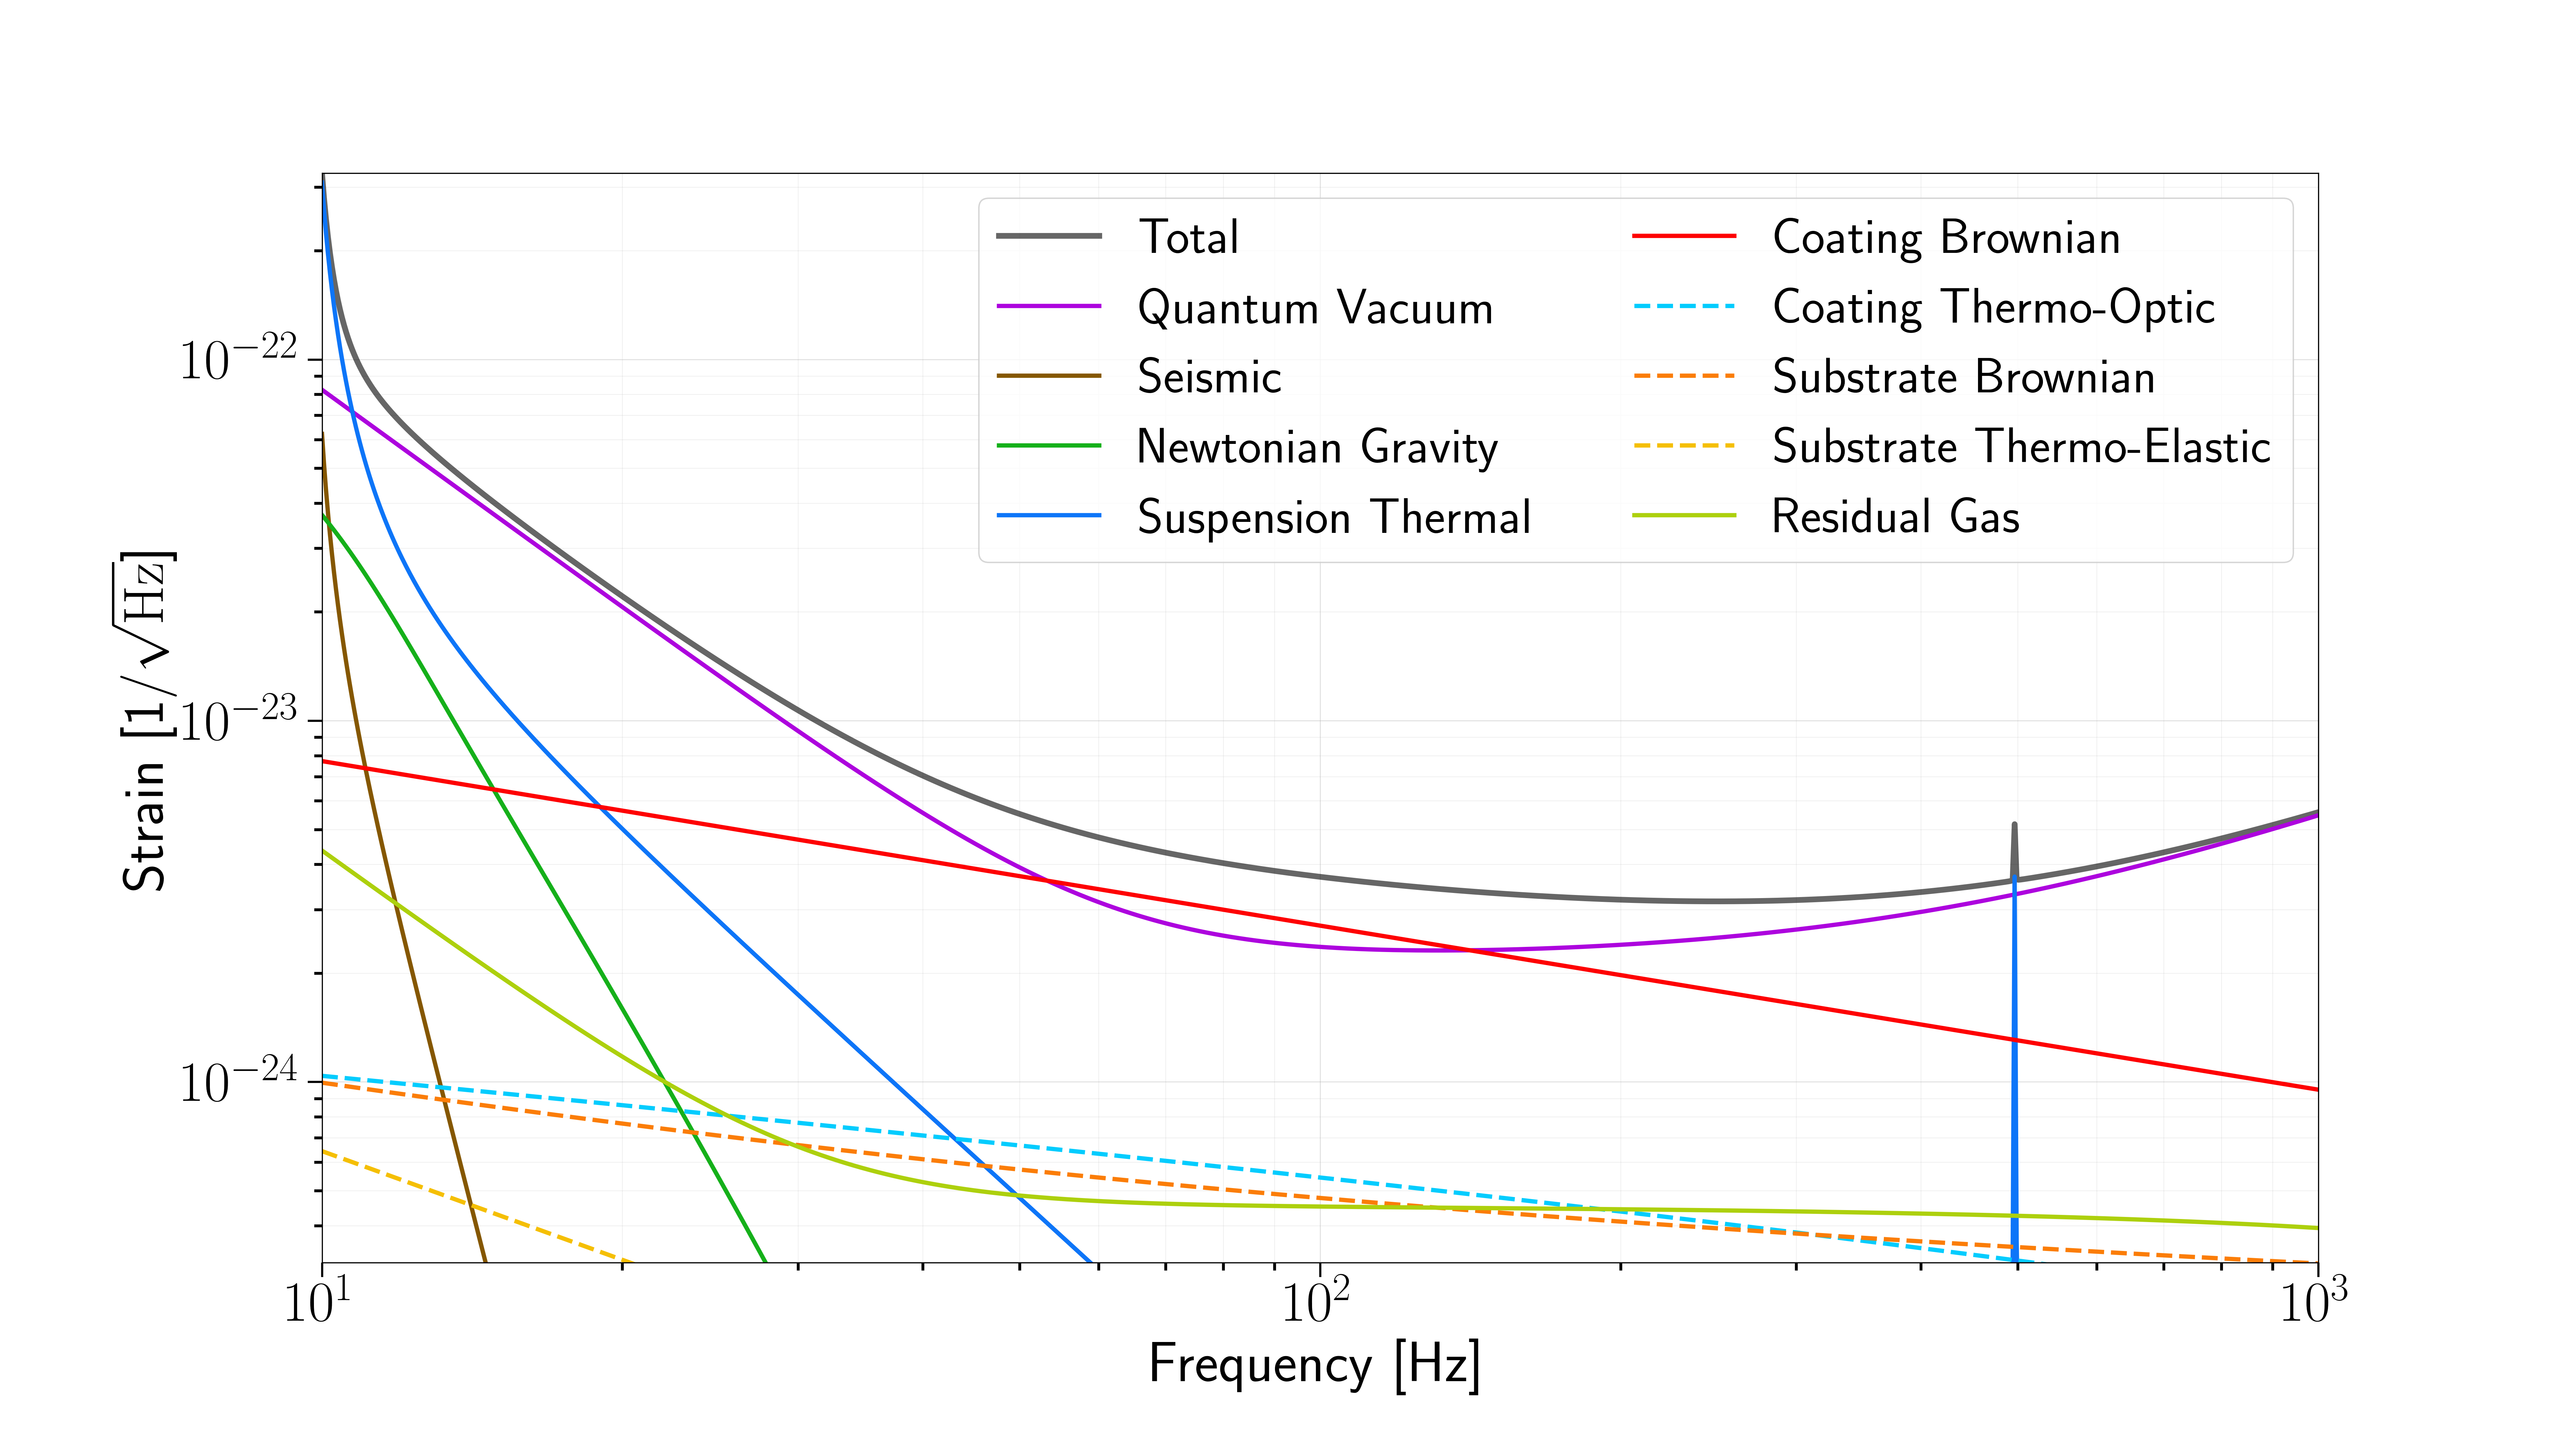
\includegraphics[width=\textwidth]{figs/ALGAAS/aligo_budget_gwinc.png}
\end{center}
\caption{ALIGO noise budget placeholder for silica-tantala, and gaas-algaas brownian noise comparison}
\label{fig:aligo_tn_comparison}
\end{figure}

\subsubsection{$\mathrm{SiO_2}/\mathrm{TiO_2:Ta_2O_5}$ coating parameters}
Currently the LIGO interferometers deposit $\lambda$/4 stacks of silica and titania doped tantala on fused silica test mass substrates. Effective loss angle measurements \cite{Harry:06}

\textbf{Current $\mathrm{SiO_2}/\mathrm{TiO_2:Ta_2O_5}$ elasticity params, power spectra, and strain spectral density (order of magnitude estimate)}

\subsubsection{$\gaas$/$\algaas$ coating parameters}
\textcolor{red}{Specific coating parameters for most promising $\algaas$ candidates? Chat with Steve. Or just mention parameters that are listed in Cole 2013}
\cite{Cole:2013}

\textcolor{red}{Insert computed curves of the most precise and recent (effective) loss angle measurements (Nick Demos measurements?). More instructive to plot strain spectral density or displacement power spectra}

\noindent Currently thermal noise from the $\mathrm{SiO_2}/\mathrm{TiO_2:Ta_2O_5}$ optical coatings is the largest contributor of Brownian noise in LIGO compared to estimated substrate and suspension thermal noise \cite{Harry:06}. As of the end of O3, Brownian thermal noise is estimated to be ? orders of magnitude below the current sensitivity and it will prove to be the limiting source of noise as that sensitivity is increased with various other upgrades mitigating fundamental and technical noise. (\textcolor{red}{already mentioned in intro prior to this thermal noise section. Need to re-iterate in more detail?})

\subsection{Anisotropic media}
Unlike with isotropic media, we cannot assume that the index of refraction of anisotropic media is the same for all chosen wave vectors. This is a direct consequence of the birefringence of anisotropic media; characterized by the dielectric, permittivity, and polarization tensors.

\subsubsection{The Dielectric tensor}
Further elaborating on the nature of a generalized dielectric tensor for any wavevector is required to proceed:
\begin{equation}\label{eq:3.11}
D_i = \varepsilon_{ij}E_j
\end{equation}
Where D is the displacement vector and E is the electric field vector and $\varepsilon$ is the dielectric tensor. The displacement vector for isotropic media is retrieved when $i = j$ and $\varepsilon_i = \varepsilon$. To further understand the nature of the dielectric tensor we assert Poynting's theorem providing an energy conservation requirement:
\begin{equation}\label{eq:3.12}
\nabla \cdot \vec{S} = \frac{dU}{dt}
\end{equation}
Where $\vec{S} = \vec{E} \times \vec{H}$ is the poynting vector and $U = \frac{1}{8 \pi} \big( \vec{E} \cdot \vec{D} + \vec{B} \cdot \vec{H} \big)$ is the electromagnetic field density. The reader is left to perform the exercise and show that in order for \ref{eq:3.12} to hold true given \ref{eq:3.11}


\begin{equation}
\varepsilon_{ij} = \varepsilon_{ji}
\end{equation}
Demonstrating that the dielectric tensor is symmetric - exhibiting only six unique terms. Diagonalizing the tensor, the presence of two unique eigenvectors and eigenvalues indicates the existance of two eigenpolarizations with paired eigenindices.
%The most general form of the energy density can be geometrically represented as ellipsoid but a coordinate transformation we can diagonalize and realize the principal axes of the dielectric allowing a simpler form of the displacement, and in turn the energy density.

\subsubsection{Monochromatic plane wave propogation}
Revisiting Maxwell's equations for simple monochromatic plane wave solution gives provides further direction on how crystalline media may effect incident light. Further elaborating, the following assumptions are made:
\begin{equation}
\vec{E} = E_o e^{(i \omega (\frac{n}{c} \vec{r}\cdot \vec{s}-t))}
\end{equation}
Where $n$ is the index of refraction, $c$ is the speed of light, $\vec{r}$ is the position vector and $\vec{s}$ is the unit wave normal.
\begin{equation}
\nabla \times \vec{H}= \frac{\partial \vec{D}}{\partial t}
\end{equation}
Where $\vec{H}$ is the magnetic field assuming the permeability $\mu$, and the generalized displacement vector $\vec{D}$ and electric field vector $\vec{E}$.
\begin{equation}
\nabla \times \vec{E} = -\mu \vec{H}
\end{equation}
Reducing to only the displacement and electric fields:
\begin{equation}\label{eq:3.17}
\vec{D} = \frac{n^2}{\mu}[\vec{E}-\vec{s}(\vec{s}\cdot \vec{E})]
\end{equation}
Maxwell's equations show that the electric field is not necessarily parallel to the displacement field and in most materials with non-zero polarizability tensors and dielectric tensors, it is not. But as specified above, the displacement vector, Electric field and unit wave normal are co-planar while remaining orthogonal to $\vec{H}$. Assuming we are operating within a coordinate system aligned with the principal dielectric axes, we substitute \ref{eq:3.11} into \ref{eq:3.17}:
\begin{equation}\label{eq:3.18}
E_i = \frac{n^2 s_i (\vec{E}\cdot\vec{s})}{n^2 - \mu \varepsilon_i}
\end{equation}

From here it can be shown that for a general plane wave there exist two unique refractive index solutions within the constructed dielectric. Though using this result to show this requires revisiting geometrical conditions that are best visualized using a method introduced in the next section. \textcolor{red}{For a more rigorous proof, see Appendix H in} \cite{nye}

\subsubsection{Indicatrix}\label{sec:indicatrix}
Acquiring solutions of the two indices along with the corresponding directions of propogation in the crystal for a general plane wave with unit wave vector $\vec{s}$ can be done via a conveniant geometrical construction. The construction begins by considering a constant electric energy density ($U_e$) surface in the $\vec{D}$ space; an ellipsoid is formed:

\begin{equation}\label{eq:lagr1}
\frac{D_x}{\varepsilon_x} + \frac{D_y}{\varepsilon_y} + \frac{D_z}{\varepsilon_z} = 2 U_e \varepsilon_o
\end{equation}
With redefined coordinates $(\vec{D}/\sqrt{2 U_e \varepsilon_o}) \rightarrow \vec{r}$ and setting $\varepsilon_i = n^2_i$:
\begin{equation}
\frac{x^2}{n_x^2} + \frac{y^2}{n_y^2} + \frac{z^2}{n_z^2} = 1
\end{equation}
This equation for the ellipsoid is known as the indicatrix. Given the co-planar solution demonstrated in the last section, we can impose the normal of the plane $\vec{r} \cdot \vec{s} = 0$:

\begin{equation}\label{eq:lagr2}
\vec{r} \cdot \vec{s} = x s_x + y s_y + z s_z = 0
\end{equation}
Equations \ref{eq:lagr1} and \ref{eq:lagr2} both contribute constraints to the method of finding extrema using Lagrange multipliers for the function:
\begin{equation}
r^2 = x^2 + y^2 + z^2
\end{equation}
The Lagrangian ($\mathcal{L}$) with the introduced multiplers ($\lambda_1$, $\lambda_2$) then becomes:
\begin{equation}
\mathcal{L}(\textcolor{red}{\vec{r},\vec{s}},\lambda_1, \lambda_2) =
x^2 + y^2 + z^2 + \lambda_1 (xs_x + ys_y + zs_z) + \lambda_2 \bigg( \frac{x^2}{\varepsilon_x} + \frac{y^2}{\varepsilon_y} + \frac{z^2}{\varepsilon_z} - 1 \bigg)
\end{equation}
With the generated system of equations from the Lagrange multipler method ($\partial F_i/ \partial x_i = 0$, and $\partial F_j/ \partial \lambda_j$) where index $i =x,y,z$ and $j = 1,2$ we obtain a system of 3 equations:
\begin{equation}
i \bigg(1-\frac{r^2}{\varepsilon_{i}} \bigg) + s_{i} \bigg(\frac{x s_x}{\varepsilon_x} + \frac{y s_y}{\varepsilon_y} + \frac{z s_z}{\varepsilon_z} \bigg) = 0
\end{equation}
The result is verified when substituting $r \rightarrow \frac{\vec{D}}{\sqrt{\vec{E} \cdot \vec{D} \varepsilon_o}}$ back which recovers \ref{eq:3.18}.
\\

\begin{figure}[H]
\begin{center}
\includegraphics[width=75mm]{figs/ALGAAS/indicatrix_nye.pdf}
\end{center}
\caption{General ellipsoid indicatrix with a general propogation direction (Using Nye's figure as placeholder as of now)}
\label{fig:general_indicatrix}
\end{figure}

\subsection{$\gaas$ and $\algaas$ crystal classification}
The space group of $\gaas$ as well as $\algaas$ are within the $F\bar{4}3m$ space group. Crystals of this particular space group are commonly known as zincblende crystals; a common crystal configuration named after zinc sulfide (ZnS). Cubic crystals by their crystallographic structure display optically isotropic characteristics when  stress free and no DC and/or slowly varying electric fields are present.
\satoshi{Is this true?} \textcolor{blue}{Yes. Though the birefringence seen from HR $\gaas$ coatings is said to be due to an ``intrinsic stress" in the high and low index layers. (What is breaking the symmetry to cause this? Heteroepitaxy? Annealing? Defects? Is this birefringence the same for all samples?) I think a dedicated high precision birefringence measurement on multiple samples would be cool.}

\begin{figure}[H]
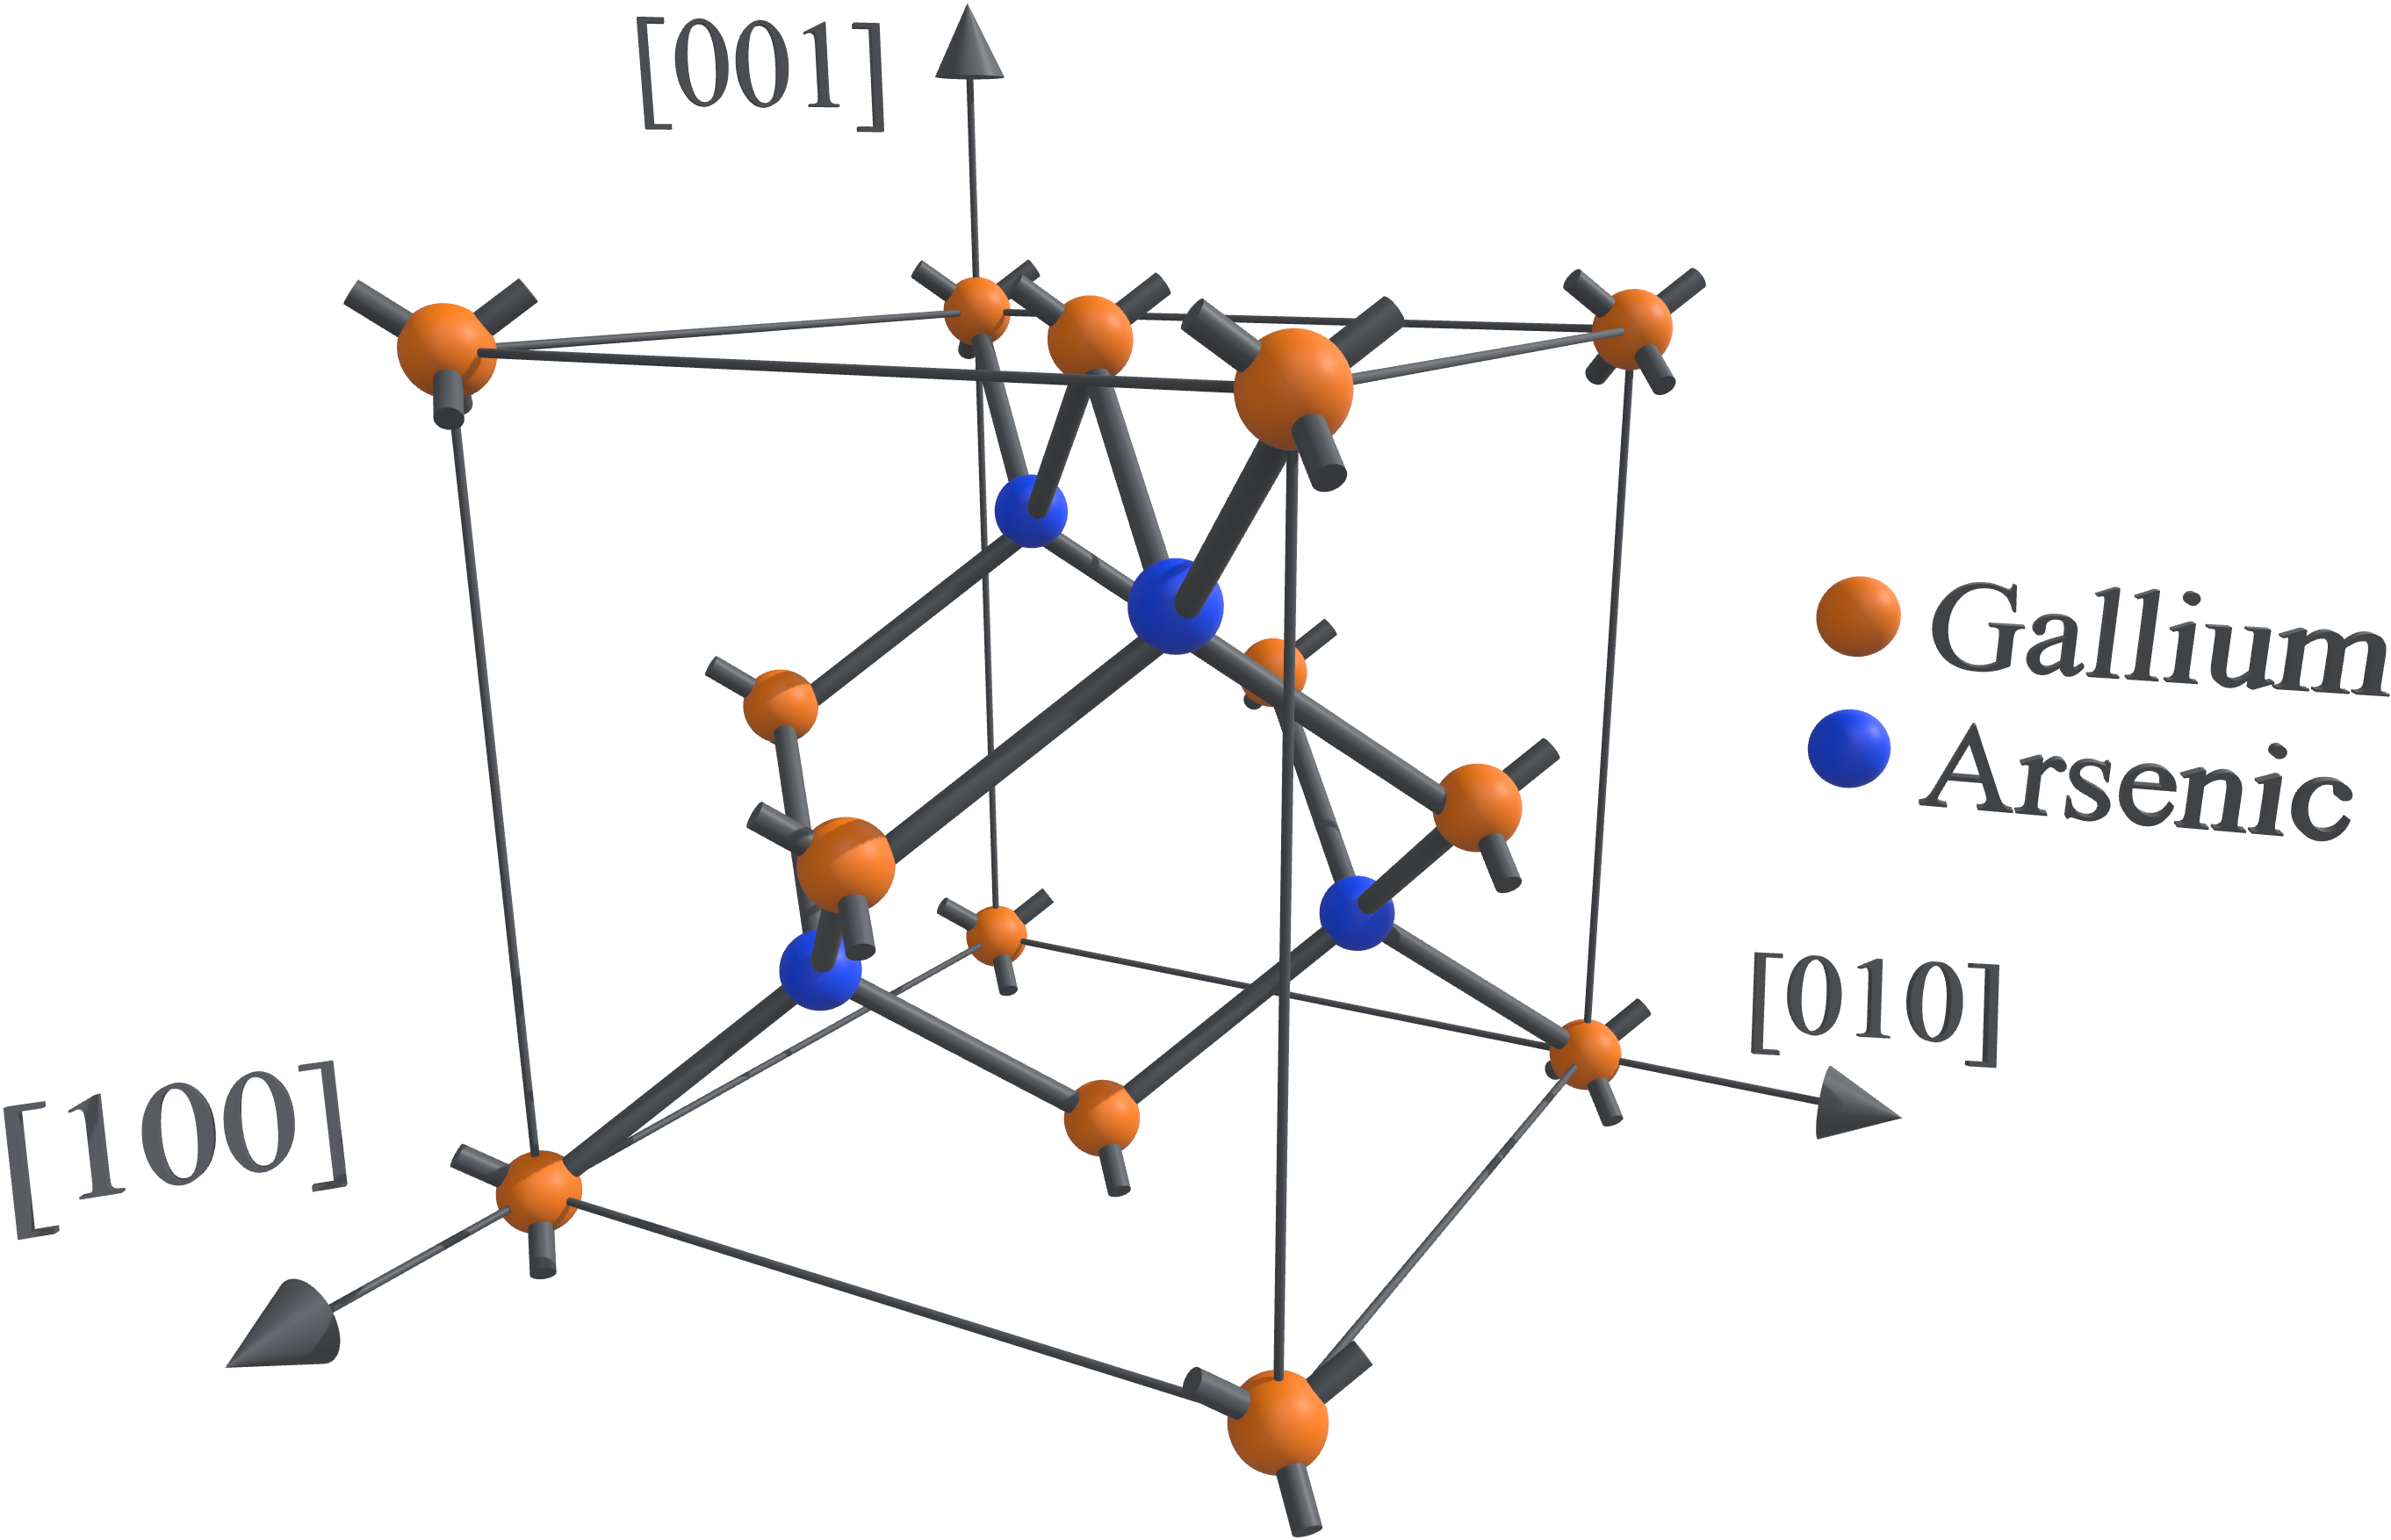
\includegraphics[width=\textwidth]{figs/ALGAAS/gaas_unit_cell_mi.PNG}
\caption{The unit cell of gallium arsenide (GaAs) with associated miller indices as coordinate axes}
\label{fig:gaas_uc}
\end{figure}

\textcolor{red}{Mention the difference in lattice cell constant between $\gaas$ and $\algaas$?}


\subsection{Induced anisotropy in zincblende crystals}
Zincblende structures, like the crystalline materials in question can exhibit birefringent properties when under the influence of two factors: stress in the material, and present within DC electric fields. These two properties of crystalline materials are known as the photoelastic and electro-optic effects respectively.

\subsubsection{The (linear) electro-optic effect}

For non-centrosymmetric crystalline media there exists a non-zero rank 2, $6 \times 3$ tensor ($r_{ij}$) connecting a slowly varying electric field $\vec{E}(f) = [E_x(f), E_y(f), E_z(f)]$ directly to the \hyperref[sec:indicatrix]{indicatrix} ~\cite{yariv,nye}:
\begin{equation}
  \left[ {\begin{array}{c}
   \big( \frac{1}{\Delta n ^2 } \big)_1 \\
   \big( \frac{1}{\Delta n ^2 } \big)_2 \\
   \big( \frac{1}{\Delta n ^2 } \big)_3 \\
   \big( \frac{1}{\Delta n ^2 } \big)_4 \\
   \big( \frac{1}{\Delta n ^2 } \big)_5 \\
   \big( \frac{1}{\Delta n ^2 } \big)_6 \\
  \end{array} } \right]
  =
%
 \left[ {\begin{array}{ccc}
   r_{11} & r_{12} & r_{13}\\
   r_{21} & r_{22} & r_{23}\\
   r_{31} & r_{32} & r_{33}\\
   r_{41} & r_{42} & r_{43}\\
   r_{51} & r_{52} & r_{53}\\
   r_{61} & r_{62} & r_{63}\\
  \end{array}} \right]
 %
 \left[{\begin{array}{c}
   E_x (f)\\
   E_y (f)\\
   E_z (f)\\
 \end{array}} \right]
\end{equation}

\noindent The $i$ index runs over the terms in the indicatix equation:
\begin{equation}
\bigg(\frac{1}{\Delta n_x^2} \bigg) x^2\ + \bigg(\frac{1}{\Delta n_y^2} \bigg) y^2 + \bigg(\frac{1}{\Delta n_z^2} \bigg) z^2 + 2 \bigg(\frac{1}{\Delta n_{xz}} \bigg)xz + 2 \bigg(\frac{1}{\Delta n_{yz}} \bigg)yz + 2 \bigg(\frac{1}{\Delta n_{xy}} \bigg)xy = 1
\end{equation}

\noindent \textcolor{red}{Detail on some prior knowledge of $f \leq f_\mathrm{max}$? (Pockels cell specs?)}

\subsubsection{$r_{ij}$ for zincblende crystals ($r_{\bar{4}3m, ij}$)}

The form of the electro-optic tensor for zincblende crystals (including $\gaas$ and $\algaas$) reduces such that $r_{ij} = r_{41} = r_{52} = r_{62} \neq 0$ with all other terms being zero:

\begin{equation}
r_{\bar{4}3m,ij} =
 \left[ {\begin{array}{ccc}
  0 & 0 & 0\\
  0 & 0 & 0\\
  0 & 0 & 0\\
  r_{41} & 0 & 0\\
  0 & r_{52} & 0\\
  0 & 0 & r_{63}\\
 \end{array}} \right]
\end{equation}

\noindent Where also $r_{41} = r_{52} = r_{63}$

\subsubsection{New principal (electro-optic) dielectric axis for zincblende structures}

In general the principle dielectric axes of the new ellipsoid do \textbf{not} coincide with the axes of the ellipsoid of the unperturbed crystal. The form of the index ellipsoid for a zincblende crystalline material accounting for the electro-optic tensor and some generalized DC electric field $\vec{E}$ expressed in terms of the crystallographic axes is given by:
\begin{equation}\label{eq:zindicatrix}
\bigg(\frac{1}{n_o^2} \bigg) x^2\ + \bigg(\frac{1}{n_o^2} \bigg) y^2 + \bigg(\frac{1}{n_o^2} \bigg) z^2  + 2r_{41} E_{[100]} yz + 2r_{41} E_{[010]} xz + 2r_{41}E_{[001]} xy= 1
\end{equation}

\noindent Where we have set $n_x = n_y = n_z = n_o$ for zincblende structures.

\noindent The two principal axes are given by the eigenvectors of the the matrix given from the equation above:

\begin{equation}
 \left[ {\begin{array}{ccc}
   \big( \frac{1}{n_o ^2} \big)& r_{41}E_{[001]} & r_{41} E_{[010]}\\
   r_{41}E_{[001]} & \big( \frac{1}{n_o ^2} \big) &  E_{[100]}\\
   r_{41} E_{[010]} & r_{41} E_{[100]} & \big( \frac{1}{n_o ^2} \big)\\
  \end{array}} \right]
\end{equation}

\subsubsection{The photoelastic effect?}

When a general strains $S_{kl}(r) = \frac{1}{2} \bigg[ \frac{\partial u_k (r)}{\partial x_i} + \frac{\partial u_i (r)}{\partial x_k} \bigg]$ are applied to a material, the photoelastic tensor $p_{idkl}$ relates to the indicatrix by the following relation:

\begin{equation}
 \bigg( \frac{1}{\Delta n^2} \bigg)_{id} = p_{idkl} S_{kl}
\end{equation}

\textcolor{red}{Supplementary comment to the measured birefringence from the mentioned intrinsic strain of the high and low index layers}

\subsubsection{The generalized indicatrix}

\subsubsection{New principal dielectric axes for zincblende structures (zinblende photoelastic tensor, zincblende electro-optic tensor)}

\subsection{Optical anisotropy of a HR $\gaas$ / $\algaas$ stack}
The analysis of a highly reflective $\gaas$/$\algaas$ stack is the sole purpose of the introduction of the geometric tools prepared in the prior section. This section implements said tools by: 1) making considerations of crsytal coordinates when asserting an optical axis on a highly reflective crystalline stack manufactured by Thorlabs, 2) citing coating parameters and observed intrinsic birefringence from the highly reflective coating stack in question, 3) analyzing differential linear electro-optic effect on the phase of a reflected beam, and 4) estimating the the differential phase noise in LIGO based on calibrated electric field measurements.
%\subsubsection{Growth orientation (Miller indices) with respect to substrate surface}
%\begin{itemize}
%\item Mirror surface is the [100] plane.
%\item Within the [100] plane the AlGaAs coating is grown with a flat indicator that draws a line within the [0-11] plane where the bisected line points towards the sample center.
%\end{itemize}

\subsubsection{Miller indices for highly reflective coatings $\gaas$/$\algaas$ coatings}
\begin{figure}[H]
\begin{center}
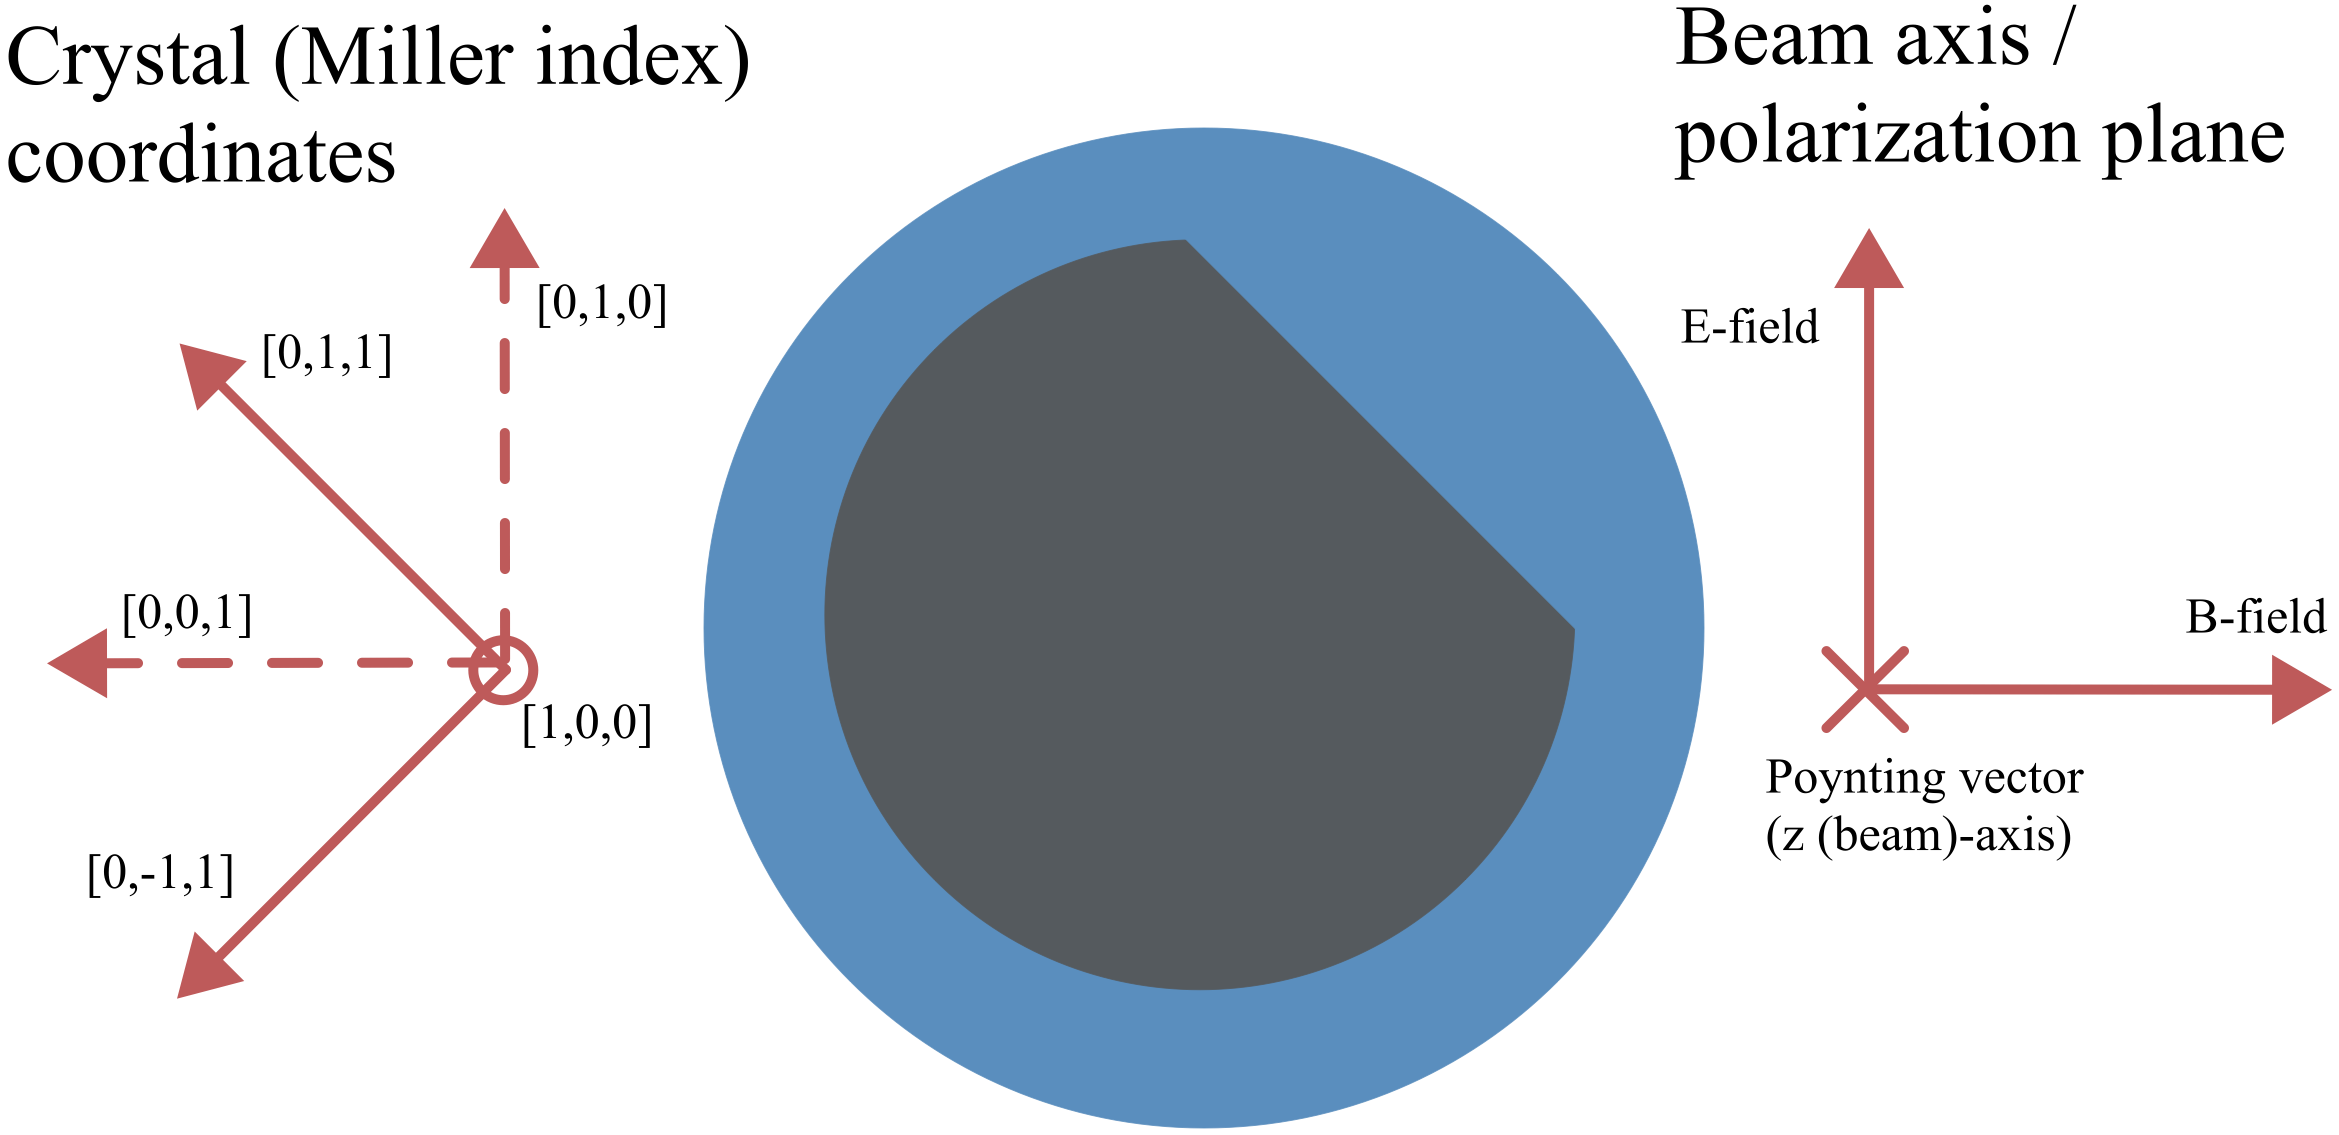
\includegraphics[width=\textwidth]{figs/ALGAAS/algaas_sample_diagram.png}
\end{center}
\caption{Figure of the beam propogation axis with respect to the AlGaAs/GaAs crystal axes (not final version). Within the [100] plane the AlGaAs coating is grown with a flat indicator that draws a line within the [0-11] plane where the bisecting vector of the plane normal points towards the sample center. The axis formed by the [100] is parallel with the beam axis (z-axis). The polarizations of incident and reflected beam oscillate along vectors within the plane formed by the normal of that axis.}
\label{fig:algaas_coords}
\end{figure}

Up until this point we have discussed three different coordinate axes: the crystal axis (indicated by Miller index plane normals), the principal dielectric axis (coordinates based in diagonalization of the indicatrix), and an optical axis (when considering a desired (laser) light propogation). We assert the beam axis \cite{fig:algaas_coords} with linearly p-polarized light.



\subsubsection{Relevant coating parameters}
\textcolor{red}{What is the variability in this coating since \cite{Cole:2013}?}
\\
\textcolor{red}{Cole 2013 coating}
\begin{itemize}
\item 81 layers ($6.83 \mu m$ thick)
\item $\gaas$ ($n_\gaas$ = 3.480)
\item $\algaas$ ($n_\algaas$ = 2.977)
\item Base coating layer of 270-nm-thick $\algaas$
\end{itemize}
\textcolor{red}{Our coating}
\\
The coating to be studied consists 36 $\lambda$/4  thick layers of $\gaas$ interspersed with 35 layers of $\lambda$/4 thick $\algaas$.   $\gaas$ forms the top and bottom layer to prevent oxygen absorption from the AlGaAs layer. The $\gaas$ layers have an index of $n_{\gaas} = 3.480$ and a thickness of $\Delta d_{\gaas} = 76.43$ nm while the low index $\algaas$ layers are $n_{\algaas} = 2.977$ with thickness $\Delta d_{\algaas} = 89.35$ nm.

%High Index:  GaAs, n=3.480, layer thickness is 76.43 nm
%Low Index:  $ \mathrm{Al}_{0.92} \mathrm{Ga}_{0.08} \mathrm{As} $, n=2.977, layer thickness is 89.35 nm
%\textcolor{red}{Info from Steve. Written source?}

\subsubsection{Electro-optic coupling to the reflected phase of a HR mirror coating}
With our coordinate considerations and established beam axis, it is now worth considering the influence of an isotropic white noise field ($E_n = [E_{nx},E_{ny},E_{nz}]$):

\begin{equation}
 \left[ {\begin{array}{ccc}
   \big( \frac{1}{n_o ^2} \big)& r_{41}E_{ny} & r_{41} E_{nx}\\
   r_{41}E_{ny} & \big( \frac{1}{n_o ^2} \big) & r_{41} E_{nz}\\
   r_{41} E_{nx} & r_{41} E_{ny} & \big( \frac{1}{n_o ^2} \big)\\
  \end{array}} \right]
\end{equation}

Assuming $E_n$ is small, the indicatrix change of $E_{nx}$ and $E_{ny}$ relative to $E_{nz}$ (as seen by the beam polarization) will be small ($r_{41}E_{n(x/y)} \ll r_{41}E_{nz}$). After diagonalizing with relevant terms \footnote{Note that the form of the tensor is still in the crystal coordinates but the $E_n$ terms are placed in the tensor such that their directions align with beam axis coordinates.} in the tensor, we are left with the following eigenindices:

\begin{equation}
\begin{aligned}
n_x' & = n_o - r_{41}E_{nz} \\
n_y' & = n_o + r_{41}E_{nz}
\end{aligned}
\end{equation}

%\textcolor{red}{How the modulation of the phase of the carrier field is dependent on the orientation of its wave vector with respect to the crystal structure, the modulating electric field direction and strength, (other items to discuss in terms of introducing the effect)}
For GaAs @ $10.6\mu$ $r_{41} = 1.6 \times 10^{-12}$ [m/V]
\\
Adachi estimate for $\mathrm{Al_{x}Ga_{1-x}As}$?
\\
\textcolor{red}{Relevant eigenpolarizations, non-optical field $E_y = E_z = 0$?}
\\
\textcolor{red}{Figure: Transformed indicatrix (Before and after $E_x$)}
\\
\textcolor{red}{Figure: Ellipse cross section. New eigenpolarizations and corresponding indices and their influence on incident field (Marty's result)}
\\
Assuming we are operating in a coordinate system suggested in \hyperref[fig:algaas_coords]{Figure ?}. Given this configuration, which plane is impacted by some $E_\mathrm{noise}$? Revisiting the \hyperref[eq:zindicatrix]{indicatrix}. We can see that for even non-zero z and y components that the only coupling to the input beam polarization is the index along the cross coupled zy axis through $E_z$ is that of the $E_x$ term. This gives us the ability to easily diagonalize the indicatrix tensor by setting the non-relevant field terms to zero.
Fejer and Bonilla take an analytical approximation approach when finding the impact of the electric field to the change in phase of the light through a crystalline anisotropic thin film ($\lambda/4$) stack \cite{bonilla_fejer}.

\begin{equation}
\hat{\phi}' = \frac{\pi n_1 z}{1-z^2}(z^{2N} -1) \frac{z^{2N} \frac{(n_f)^2}{n_2 n_3}(n_2 \kappa_{\gamma 2} + n_3\kappa_{\gamma 3}) - (n_2 \kappa_{\gamma 3} + n_3\kappa_{\gamma 3})}{(n_1)^2 -(n_f)^2 z^{4N}}
\end{equation}

with $z = \frac{n_2}{n_3}$
and
$
\kappa_{\gamma j} = \frac{d}{d \gamma} \mathrm{log}(n_j h_j)|_{\gamma =\gamma_{O}} \bigg(\frac{\hat{n}_j'}{\hat{n}_j} +\frac{\hat{h}_j'}{\hat{h}_j} \bigg)
$

With $\kappa$ being a scalar parameter.

\satoshi{Adding a schematic would be helpful.}

\textcolor{red}{Figure is in the works}

\subsubsection{Numerically friendly estimate}

In the appendix of \cite{ballmer2015} Ballmer constructs a coating layer transfer function for a given coating layer k with index $n_k$, and thickness $d_k$, defining right and left propogating modes $\Psi^{R,L}$ repsectively:

\begin{equation}
  \left[ {\begin{array}{c}
   \Psi^\mathrm{R} \\
   \Psi^\mathrm{L} \\
  \end{array} } \right]_{k+1}
  =
%
Q_k D_k
%
 \left[{\begin{array}{c}
   \Psi^\mathrm{R} \\
   \Psi^\mathrm{L} \\
 \end{array}} \right]
\end{equation}

$D_k$ applies the phase ($\phi_k = 4\pi n_k d_k /\lambda_0$) from a given coating layer, and $Q_k$ applies the transfer function between high-low/low-high index layers transition:

\begin{equation}
Q_k = \frac{1}{2n_{k+1}}
\left[ {\begin{array}{cc}
  n_{k+1} + n_k & n_{k+1} - n_k\\
 n_{k+1} - n_k & n_{k+1} + n_k\\
\end{array} } \right]
\end{equation}

\begin{equation}
D_k = \frac{1}{2n_{k+1}}
\left[ {\begin{array}{cc}
  e^{-i \phi_k / 2}& 0\\
 0 & e^{i \phi_k / 2}\\
\end{array} } \right]
\end{equation}
Defining a HR coating stack, the total transfer matrix from vaccum $Q_0$ to the $N$th coating layer is:
\begin{equation}
M = Q_N D_N ...Q_kD_k...Q_1D_1Q_0
\end{equation}

The impact of a differential electric noise field ($E$) on $M$ due to the electro-optic effect on the kth layer, we use the chain rule:

\begin{equation}
\frac{\partial M}{\partial E}  = \frac{\partial M}{\partial \phi_k} \frac{\partial \phi_k}{\partial n_k} \frac{\partial n_k}{\partial E} = Q_N D_N ...Q_kD_k?...Q_1D_1Q_0
\end{equation}


\subsection{Measured birefringence from HR $\gaas$/$\algaas$ mirrors}
There seems to be different accounts of a measured birefringence from HR $\gaas$ / $\algaas$ (\href{https://dcc.ligo.org/DocDB/0181/G2200386/001/G2200386.pdf}{Satoshi}, \href{https://nodus.ligo.caltech.edu:8081/CTN/1474}{CTN}, \href{https://dcc.ligo.org/DocDB/0181/G2200559/001/G2200559-v1%20-%20polarization.pdf}{Aidan})
\\
\textcolor{red}{Is the measured birefringence static? (Layer bonding method might introduce something?)}
\\
\textcolor{red}{Does it change from different mounting methods? (Photoelastic) (order of magnitude estimate)}
%\\
%\textcolor{red}{Electro-optic ruled out based on field measurements and relative coupling factor.}
\\
\textcolor{red}{Measurement precision of the coating birefringence? Cavity length, Polarization drifts, etc.}
\\
The measured birefringence is estimated to be caused by an intrinsic strain between the epitaxial layers of $\gaas$/$\algaas$. \cite{Cole:2013}
\\
\textcolor{red}{Marty's document about Birefringence in Crystalline mirror coatings V.8}

\section{Projected DARM coupling}
To estimate how much DARM coupling can occur, we use use a measured field spectra acquired from installed electric field meters located within LIGO Hanford Observatory EX and EY vacuum chambers. Taking the upper and the lower EFM measurements in $.3\; [\mathrm{V}/\mathrm{m}/\sqrt{\mathrm{Hz}]}$ @ 60 Hz and $4\times10^{-3}\; [\mathrm{V}/\mathrm{m}/\sqrt{\mathrm{Hz}]}$ @ 4kHz ~\cite{efm_log}.
\satoshi{I don't think these values are calibrated. According to Martynov et al. 2016, the fluctuations in the electric filed is $\sim10^{-5}\,\mathrm{[(V/m)/\sqrt{Hz}]}$.}
This along with computed estimate above allows us to create an upper limit for what this noise might be assuming incoherent fields between the end stations and a flat frequency response within LIGO's bandwidth.

\section{Experiment}
An in-air Pound-Drever-Hall ``locked" Fabry-P\'{e}rot cavity with a highly reflective $\gaas$/$\algaas$ coated sample installed and mounted in a custom designed MACOR mount / electrode assembly was designed and implemented to attempt a calibrated measurement of the Pockels effect. Details and specifications are discussed as well as relevant measurements. The discovery of unforseen driven mechanical couplings through this study have lead to an improved dual-polarization locked experimental design.

\subsection{Design}
This section details the Pound-Drever-Hall servo which is at the heart of this experiment, the schema of the servo used, a sample / electrode assembly used for a controlled electric field injection, and the estimated calibration of the measurement.

\subsubsection{PDH servo}
The Pound-Drever-Hall technique, originally imagined for laser frequency stabilization to an ultra-stable length reference; allowing the tracking of the linear phase response of an input carrier field through the resonance of said reference. The servo fully realizes the ability of an optical cavity to act as a length / frequency discriminator. The alternative cavity offset lock provides a linear response in intensity, which may be adequate for some applications but with reduced sensitivity due to the required power reduction by operating off resonance.
\begin{figure}[H]
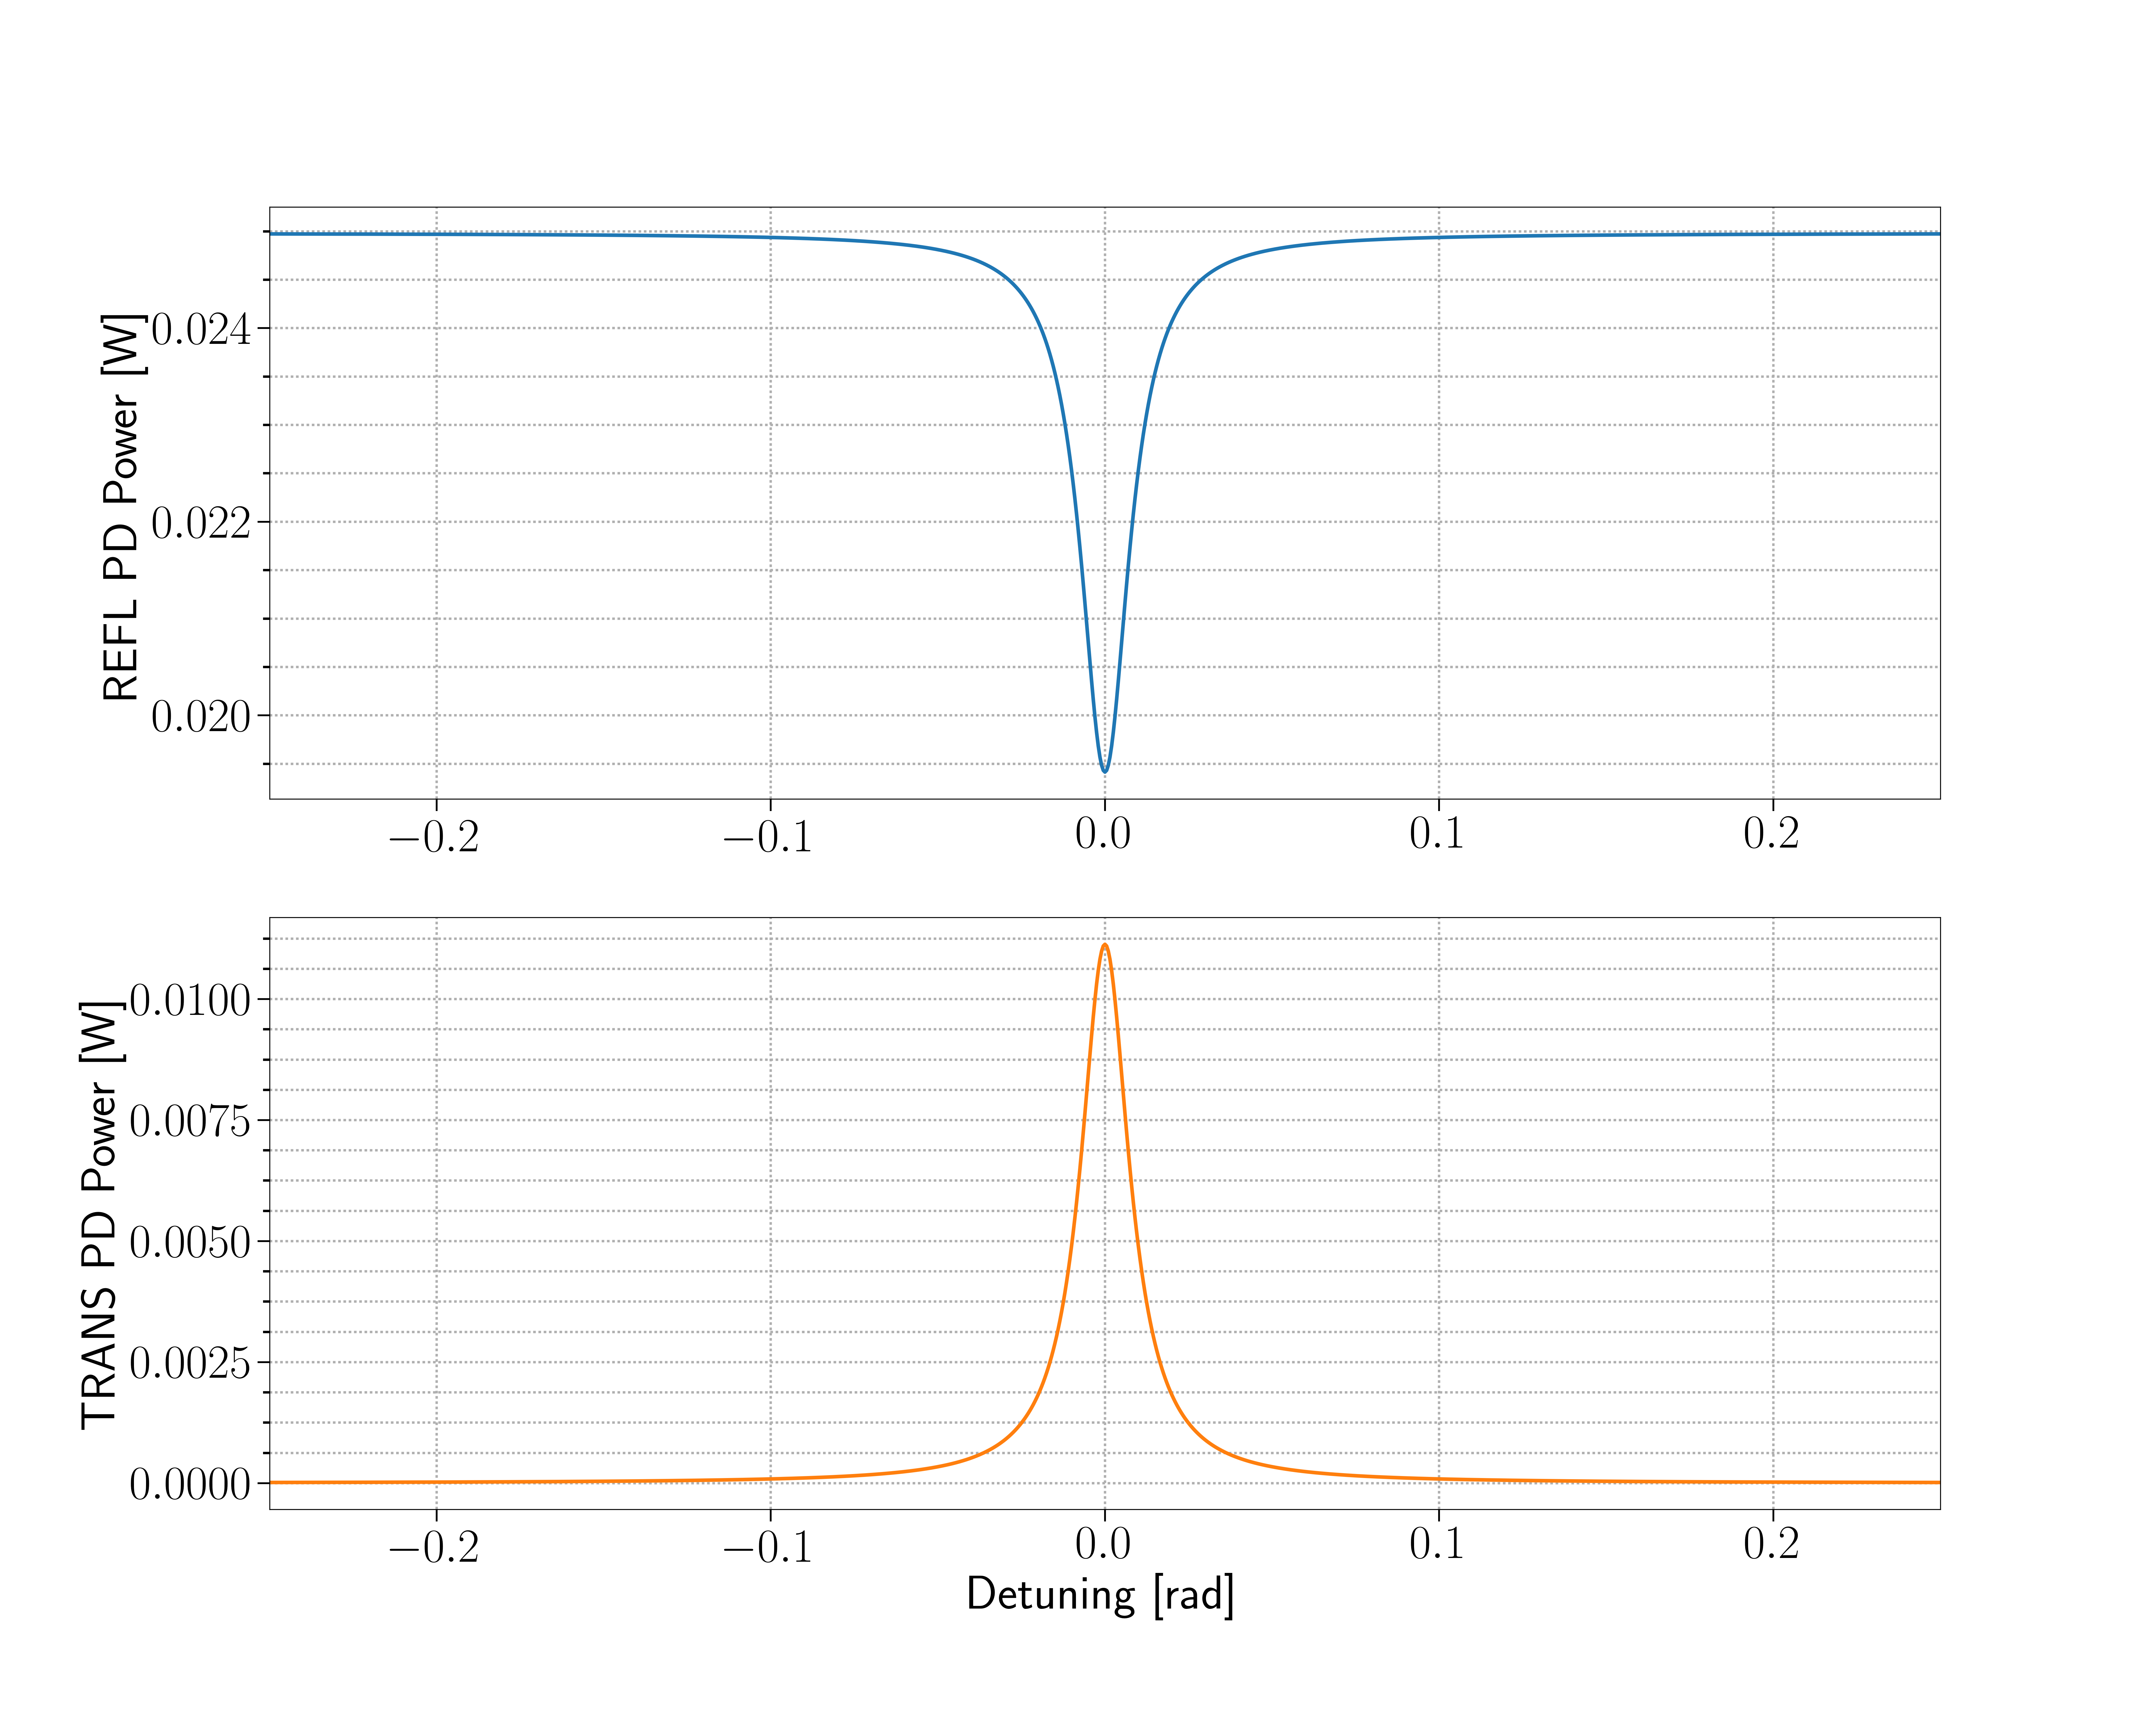
\includegraphics[width=\textwidth]{figs/ALGAAS/DC_power_cav_resonance.png}
\caption{Reflected and transmitted power around resonance.
\textcolor{red}{Phase as dotted line?}}
\label{fig:cav_length_response_DCpow}
\end{figure}
Th phase measurement is achieved by beating a separate optical field with a known frequency separation from the carrier at the cavity input. The PDH servo offers a way to avoid complicated phase-locked two laser configurations, by imposing a phase modulation on the carrier field via a Pockels cell. With high enough modulation frequency, phase modulation onto the carrier field is mathematically and physically equivalent to imposing separate optical fields (sidebands) which in most cases do not resonate in the optical cavity of interest. The modulation imposed onto the carrier is by a physically equivalent process to that mentioned in section (?). The simplified anatomy of the Pockels cell is split into three components: a crystal used to impose the modulation, capacitor plates sandwiching the crystal to introduce a controlled electric field across, and an oscillator / signal generator used to drive the capacitor at a specified frequency $\Omega$ and a voltage amplitude associated to the phase amplitude known as the modulation depth ($\beta$).

\begin{equation}
E_\mathrm{inp} = E_o e^{i \omega t + \beta \mathrm{sin}( \Omega t)}
\end{equation}

If the modulation depth is set such that $\beta < 1$ then the input field may be approximated in terms of the first two Bessel functions $J_0$, $J_1$:

\begin{equation}
E_\mathrm{inp} \approx E_0 [J_0(\beta)e^{i \omega t} + J_1(\beta)e^{i (\omega + \Omega) t} - J_1(\beta)e^{i(\omega -\Omega)t}]
\end{equation}

Setting a photodiode of area ($A_\mathrm{PD}$) in reflection of the cavity reflection coefficient of $r_\mathrm{cav}(\omega,L)$, we measure the power of the field:

\begin{equation}
 \begin{alignedat}{3}
    &P_\mathrm{refl} && \approx \frac{|E_\mathrm{refl}|^2}{A_\mathrm{PD}} && \\
    & &&\approx \frac{E_0^2}{A_\mathrm{PD}} && \bigg\{J_0^2 |r_\mathrm{cav}(\omega,L)|^2 + J_1^2(\beta)|r_\mathrm{cav}(\omega+\Omega,L)|^2 - J_1^2(\beta)|r_\mathrm{cav}(\omega-\Omega,L)|^2 +  \\
    & && && J_0J_1(\beta)\big[r_\mathrm{cav}\omega,L) r_\mathrm{cav}^*(\omega+\Omega,L)\big] - J_ 0J_1(\beta)\big[r_\mathrm{cav}(\omega,L)r_\mathrm{cav}^*(\omega-\Omega,L)\big]\bigg\}
  \end{alignedat}
\end{equation}

The two trailing terms in the above equation for $P_\mathrm{refl}$ generate a beat frequency term between the carrier and lower and upper sidebands. The magnitude and sign of these beat terms directly relate to the phase of the reflected carrier field and can be measured and transformed using specially tuned resonant electronics and a mixer into a demodulated error signal as seen in \ref{fig:pdh_error}.

\begin{figure}[H]
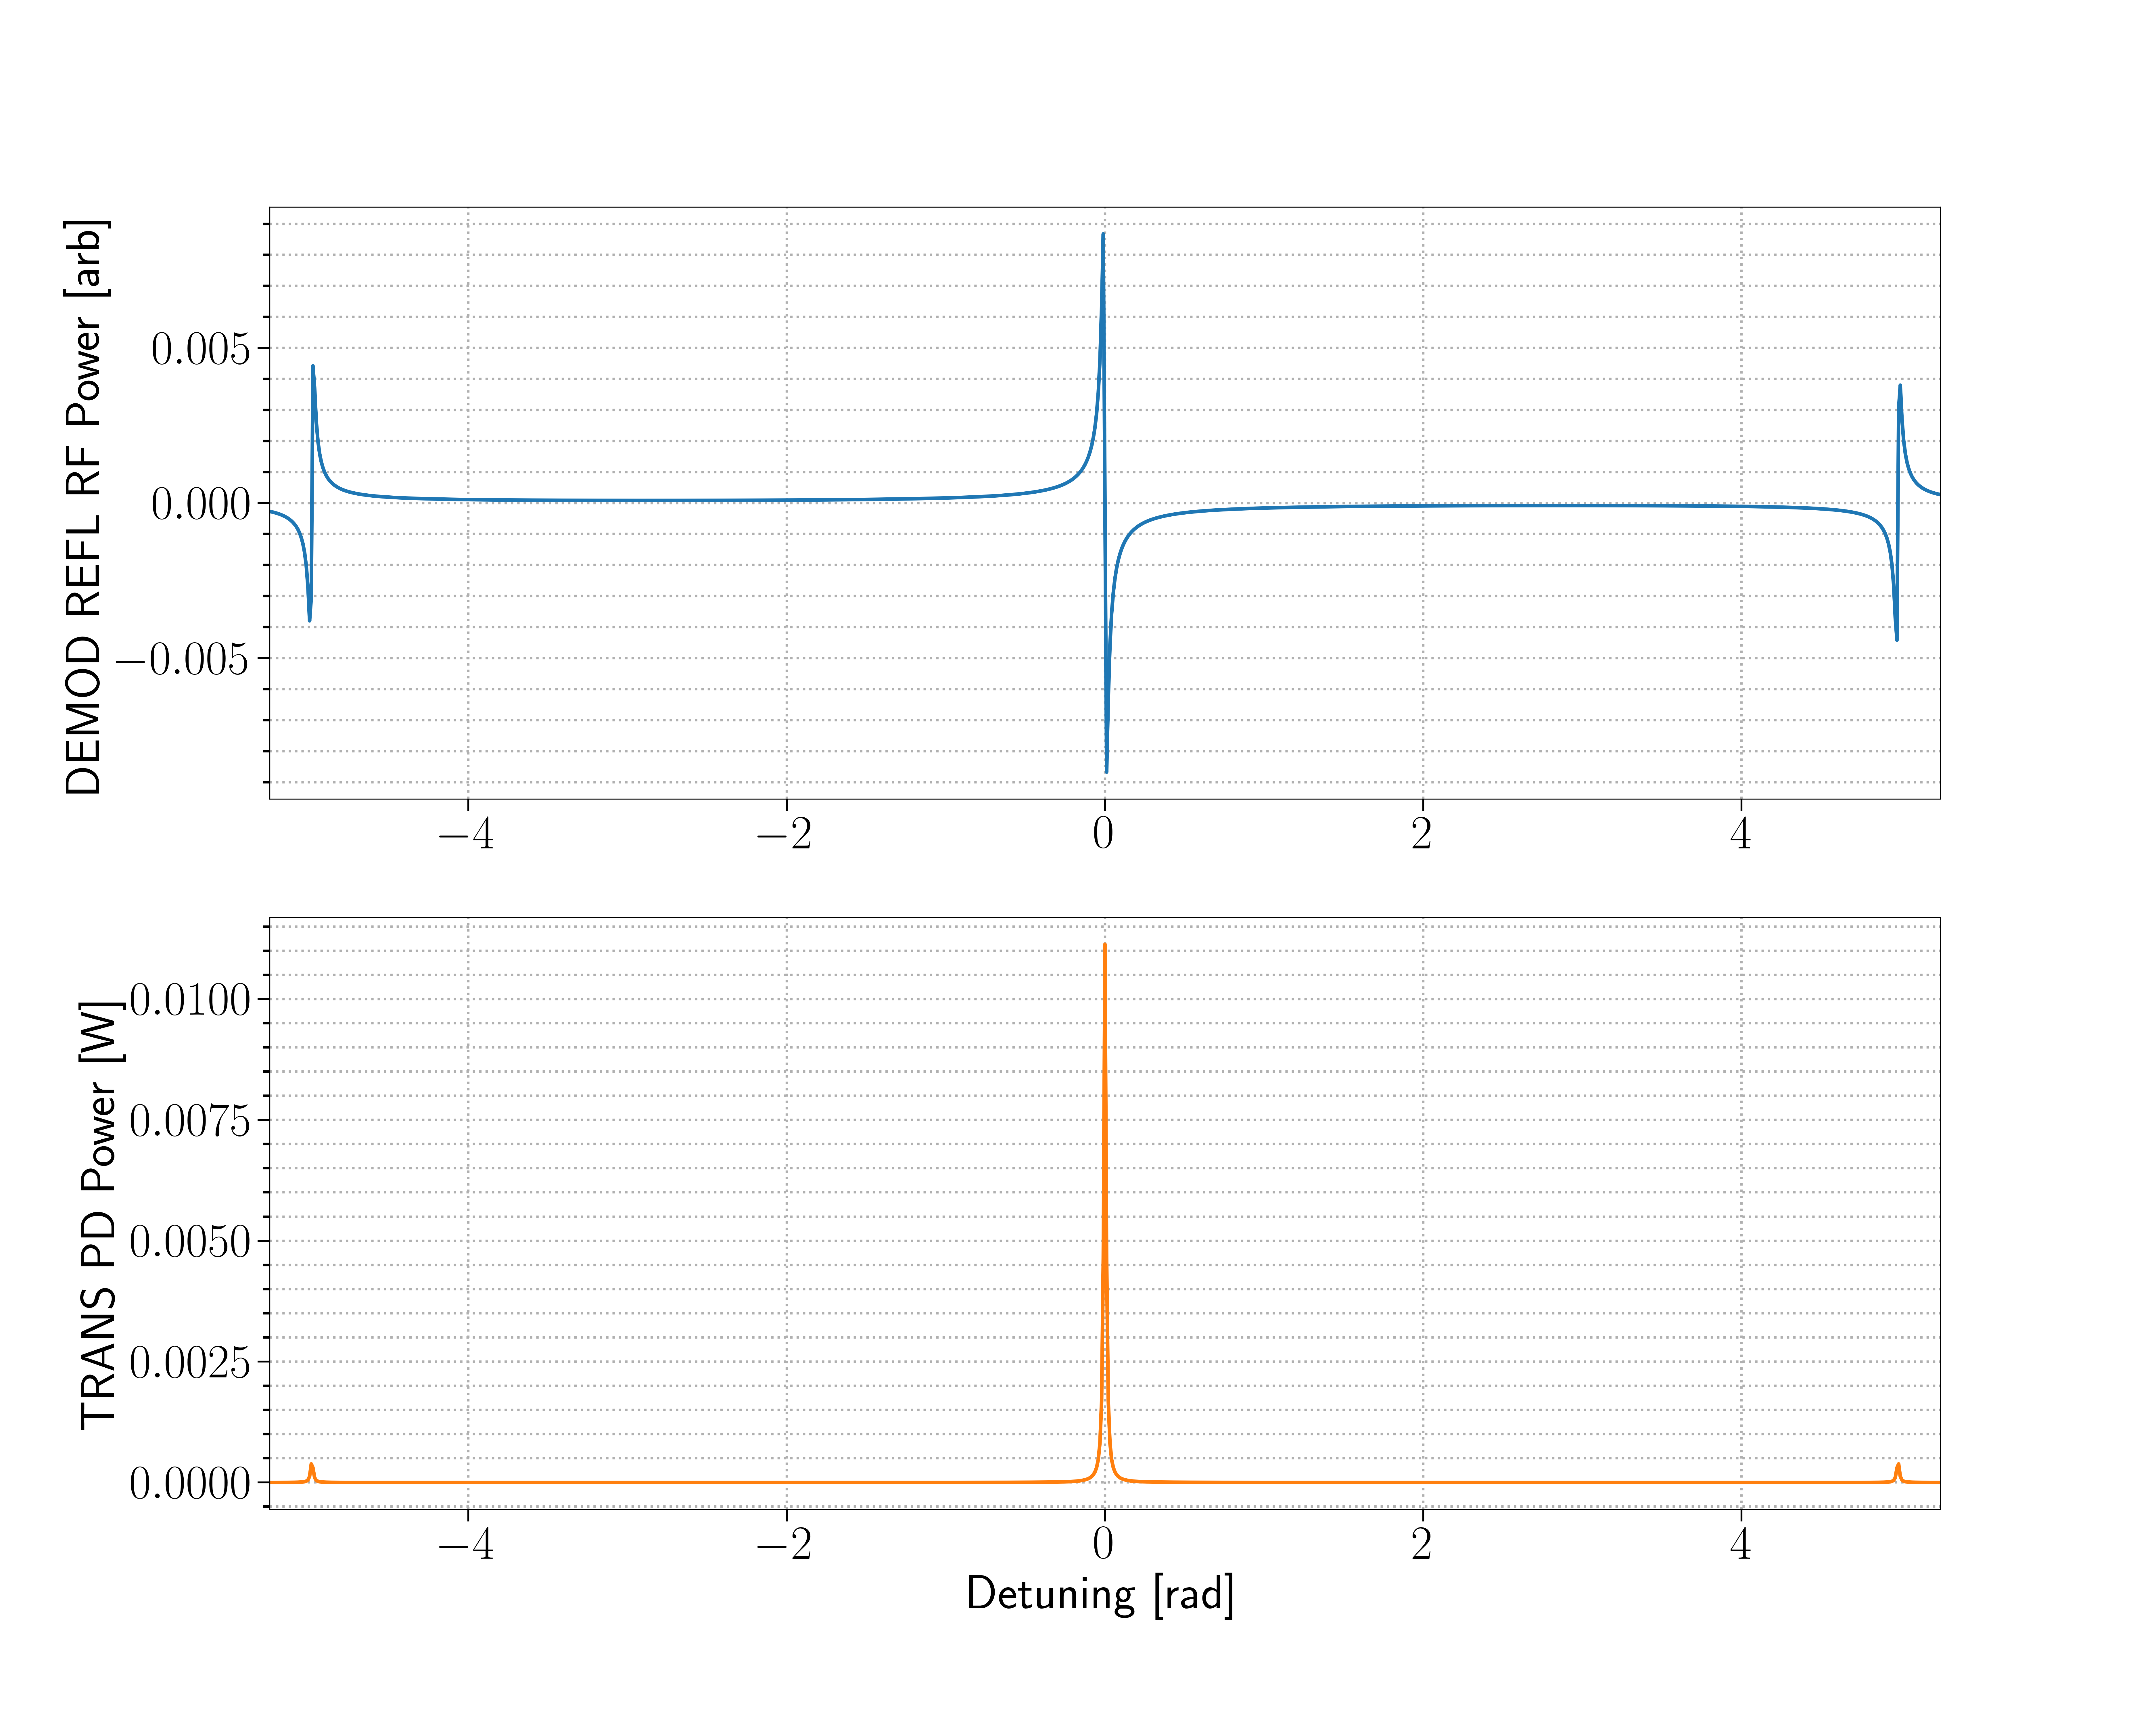
\includegraphics[width=\textwidth]{figs/ALGAAS/pdh_error.png}
\caption{By imposing 25 MHz RF sidebands we have introduced a constant reflected reference field near carrier resonance which when beat with the carrier offers a linear response after demodulating the sideband power. With the introduction of high and low frequency sideband fields, their presence is also detected through the DCPDs and PDH error signal. Their separation from resonance is equal in phase (length, and frequency) from carrier resonance.}
\label{fig:pdh_error}
\end{figure}

With this linearity and sensitivity at cavity resonance, implementation into PID feedback is the next task as any small detuning of the cavity can be registered as a drift from the loop's zero point and fed back to an actuator with an estimated calibration gain factor. When implemented into a low-noise design, this technique allows a high sensitivity measurement and calibration of a induced differential phase of the light within the stable reference cavity into differential length (or frequency).

\subsubsection{On-table schema}
\begin{figure}[H]
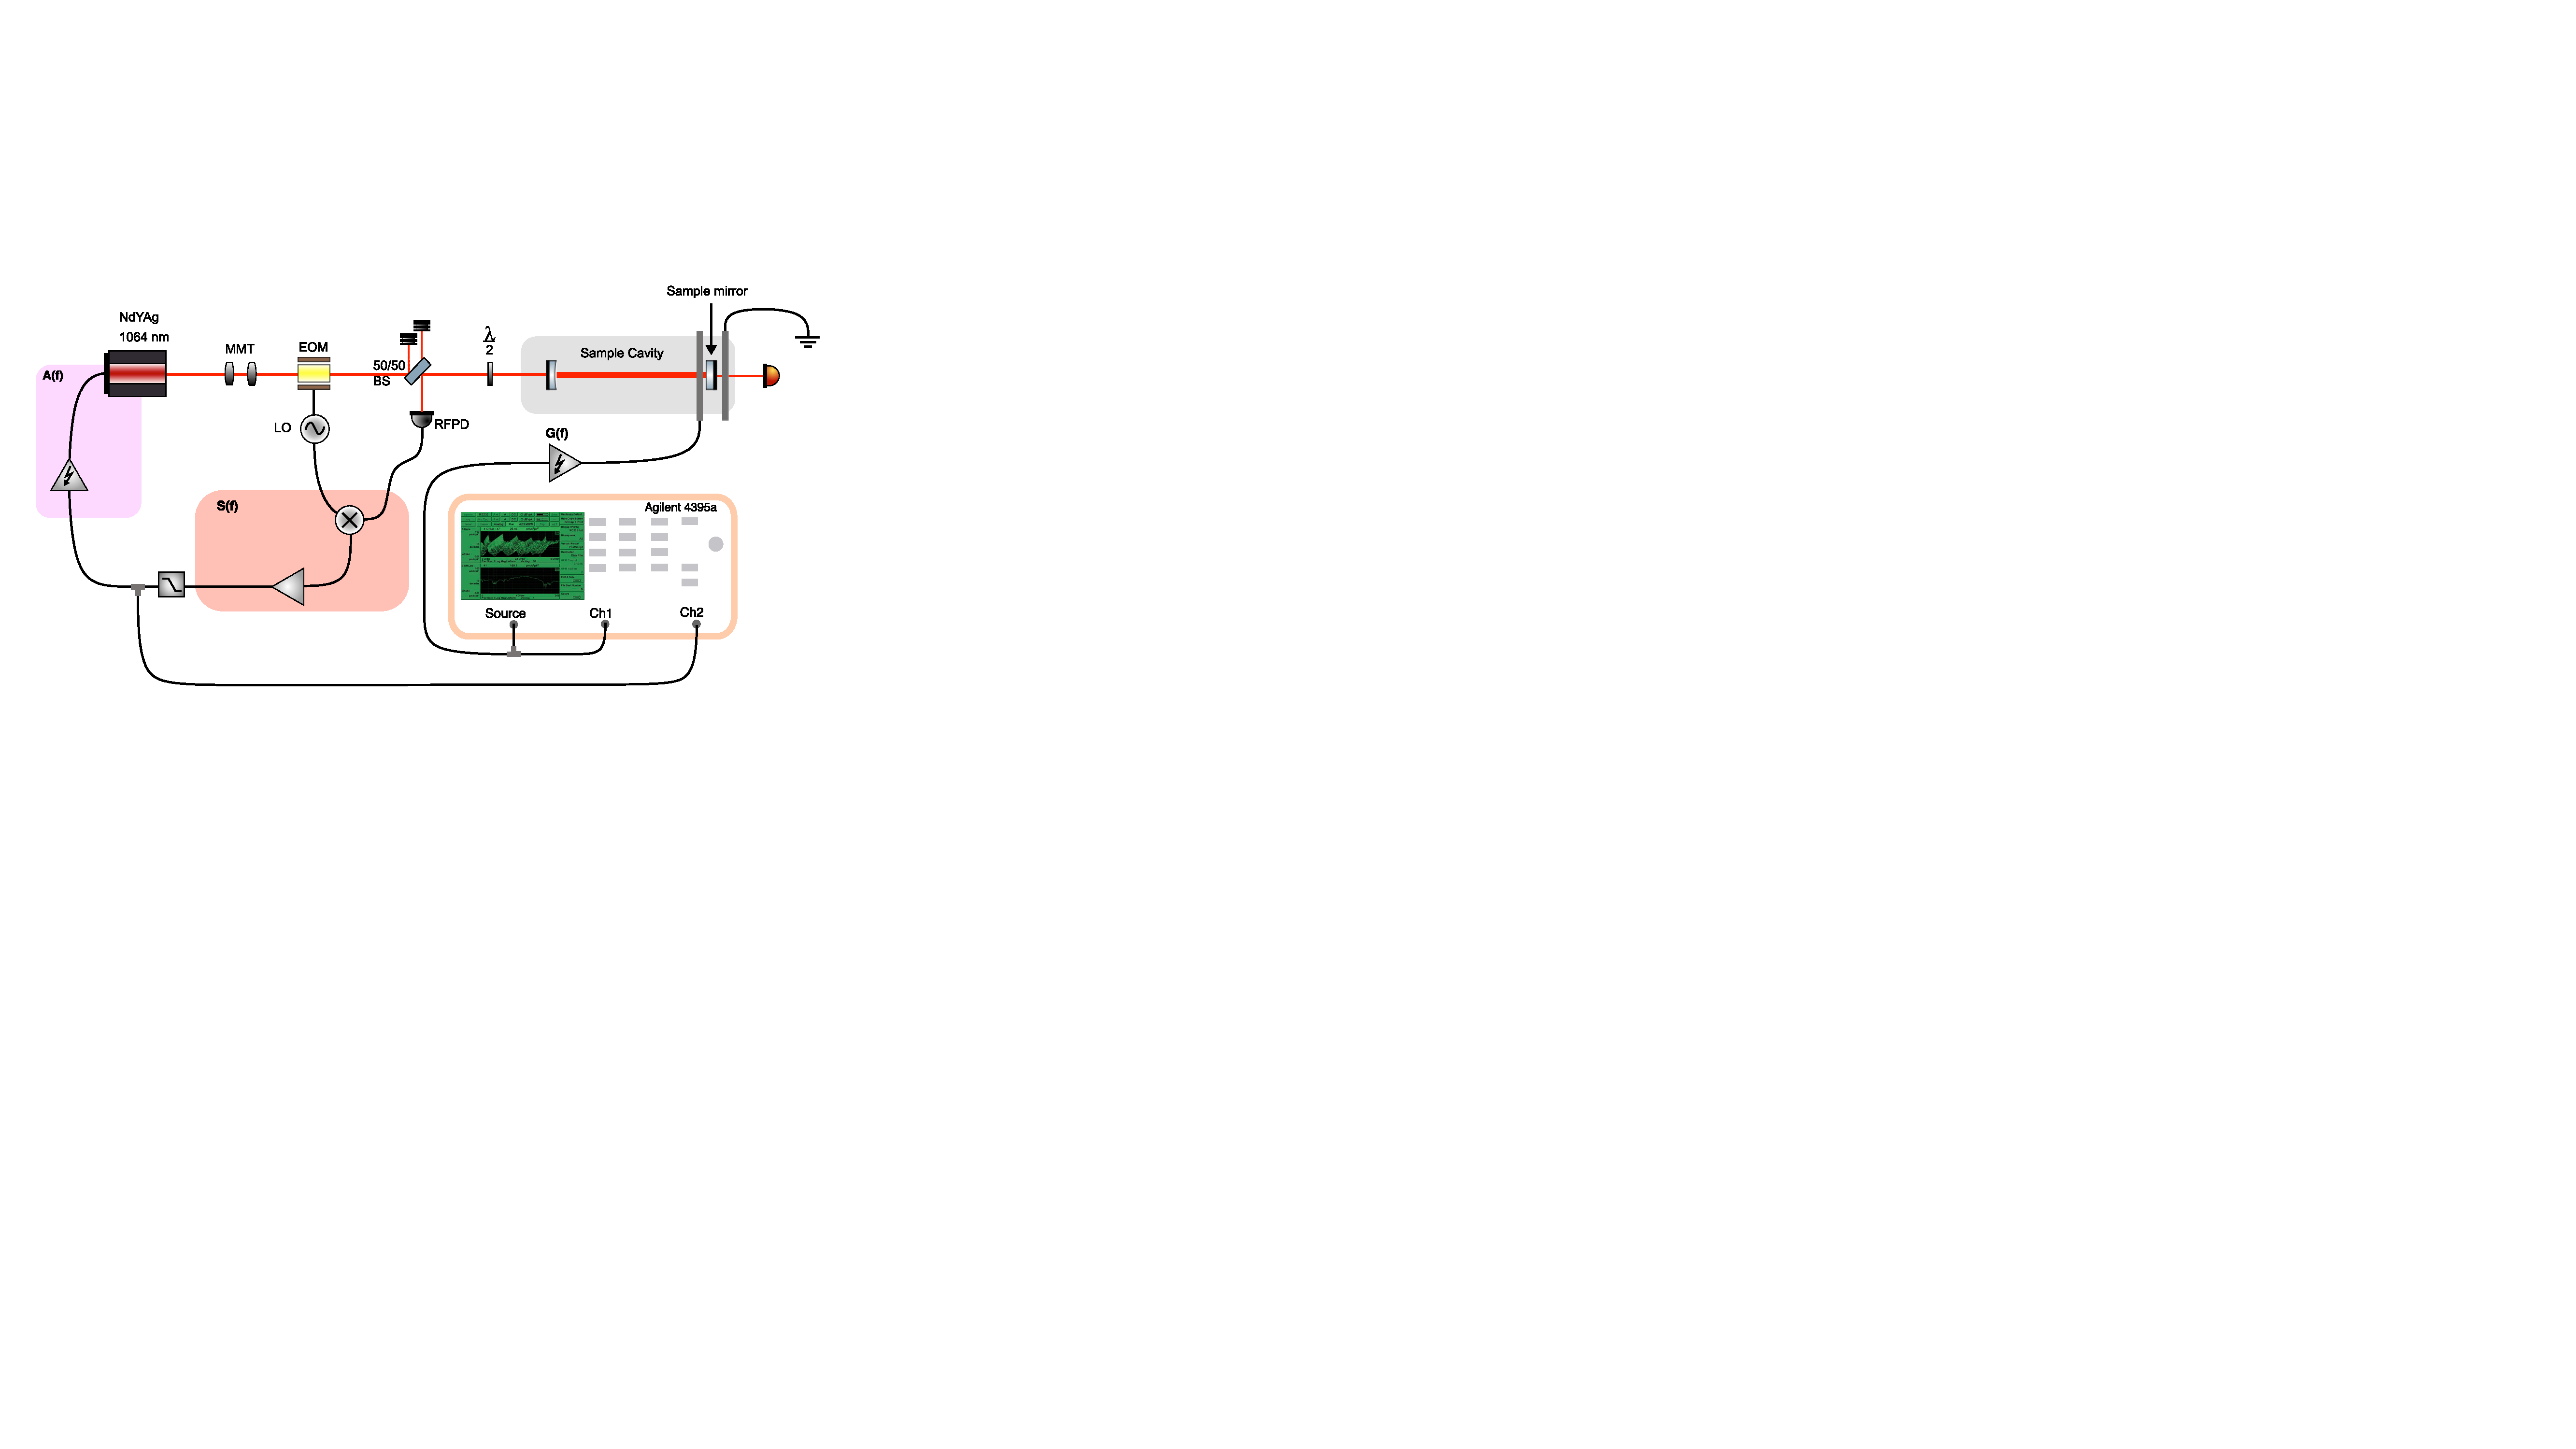
\includegraphics[width=\textwidth]{figs/ALGAAS/electrooptic_study_algaas_0.pdf}
\caption{The fundamental components of a functional PDH servo along with a pockels cell style mount design comprised of a disk capacitor sandwiching the HR AlGaAs sample, a high voltage amplifier, and a signal/network analyzer.}
\label{fig:experiment_schema}
\end{figure}

\textcolor{red}{A figure that highlights path that is intended for locking onto the PMC, and a different color highlight for the path to the experiment
The setup presented in this section, branches off of a previously established optical path used to lock onto a separate optical cavity (PMC).}
\\

The experiment designed can be decomposed into three abstractions: the servo optical plant, servo electronics, and the Pockels cell injector.
The laser light source is a Mephisto 2000 NE 1064nm laser.
\\
25 MHz EOM is a New Focus Model 4003 IR resonant phase modulator.
\\
The designed cavity is a 0.1651 m long cavity with a HR IBS coated sample (PL-CC, ROC =0.333 m) input coupler from CVI Melles-Griot and a GaAs/$\mathrm{Al_{.92}Ga_{.08}As}$ (PL-PL) fused silica substrate by the Crystalline Mirror Solutions (CMS) division of Thorlabs with the aforementioned parameters (\textcolor{red}{mentioned in coating parameters section}).

\subsubsection{Sensing S(f)}
\begin{itemize}
\item 25 MHz RFPD
\begin{itemize}
\item Transimpedance measurement (necessary? or should I just use the mixer out PDH to summarize PD/mixer response)
\end{itemize}
\item Frequency Stabilization servo (modified MIT FSS (DCCD980536)) (LTspice model in appendix)
\end{itemize}


\subsubsection{Actuation A(f)}
\begin{itemize}
\item Mephisto 2220 PZT response (capacitance estimated from HVA drive measurement with and without connection to PZT)
\item Channel 3 of SVR 350-3 BIP High Voltage Amplifier from Piezomechanik GmbH with Pomona box (elog 412)
\item \textcolor{red}{Figure of frequency response of A(f)}

\end{itemize}

\subsubsection{Low frequency servo (Thermal loop)}
\begin{itemize}
\item Passed signal from FSS $\rightarrow$ integrators $\rightarrow$ Laser thermal actuator input
\end{itemize}

\subsubsection{OLG(f)}
Isn't quite $\mathrm{A}(f)*\mathrm{S}(f)$ as stated. Doesn't entirely account for the optical plant.
How the measurement is taken (important to take between installations to account for the changes in the optical plant) (elog 831)


\subsubsection{Sample / Electrode assembly}
Maximizing the electric field ($|E_z|$) and within the coating while requiring a through beam to and through the HR coating lead us to a design very similar to that of a longitudinal pockels cell. The assembly is comprised of two disk electrodes with a 3mm central aperture. The aperture size was chosen to be at least 5 times larger than the beam size at the plate locations. This was to avoid any beam clipping while still allowing to maximize the field strength at the region of interest.
\\
Most commercial optical mounts are conductive which proved to be a problem when attempting to find a mounting solution while reducing the non-normal field gradients within the volume of interest around the sample. Because of this, we chose to construct an optical mount made of MACOR a machinable ceramic with high a high Young's modulus (66.9 GPa), and a moderate Poisson ratio (.29) \cite{macor}. An optical mount for the sample made with MACOR, along with glass bearnings .48 $\pm$ .01 cm $\diameter$  and a McMaster-Carr 8-32, 1/2" ceramic screw were used to clamp and suspend the optical sample. A 1.24" $\diameter$ hole was bored into the MACOR with a (\textcolor{red}{depth?}) depth so that there is a ? mm clearance between the front and back surface of the sample to the electrode plates.

\textcolor{red}{Figure with  the sample in-situ}
\\
\begin{figure}[H]
\centering
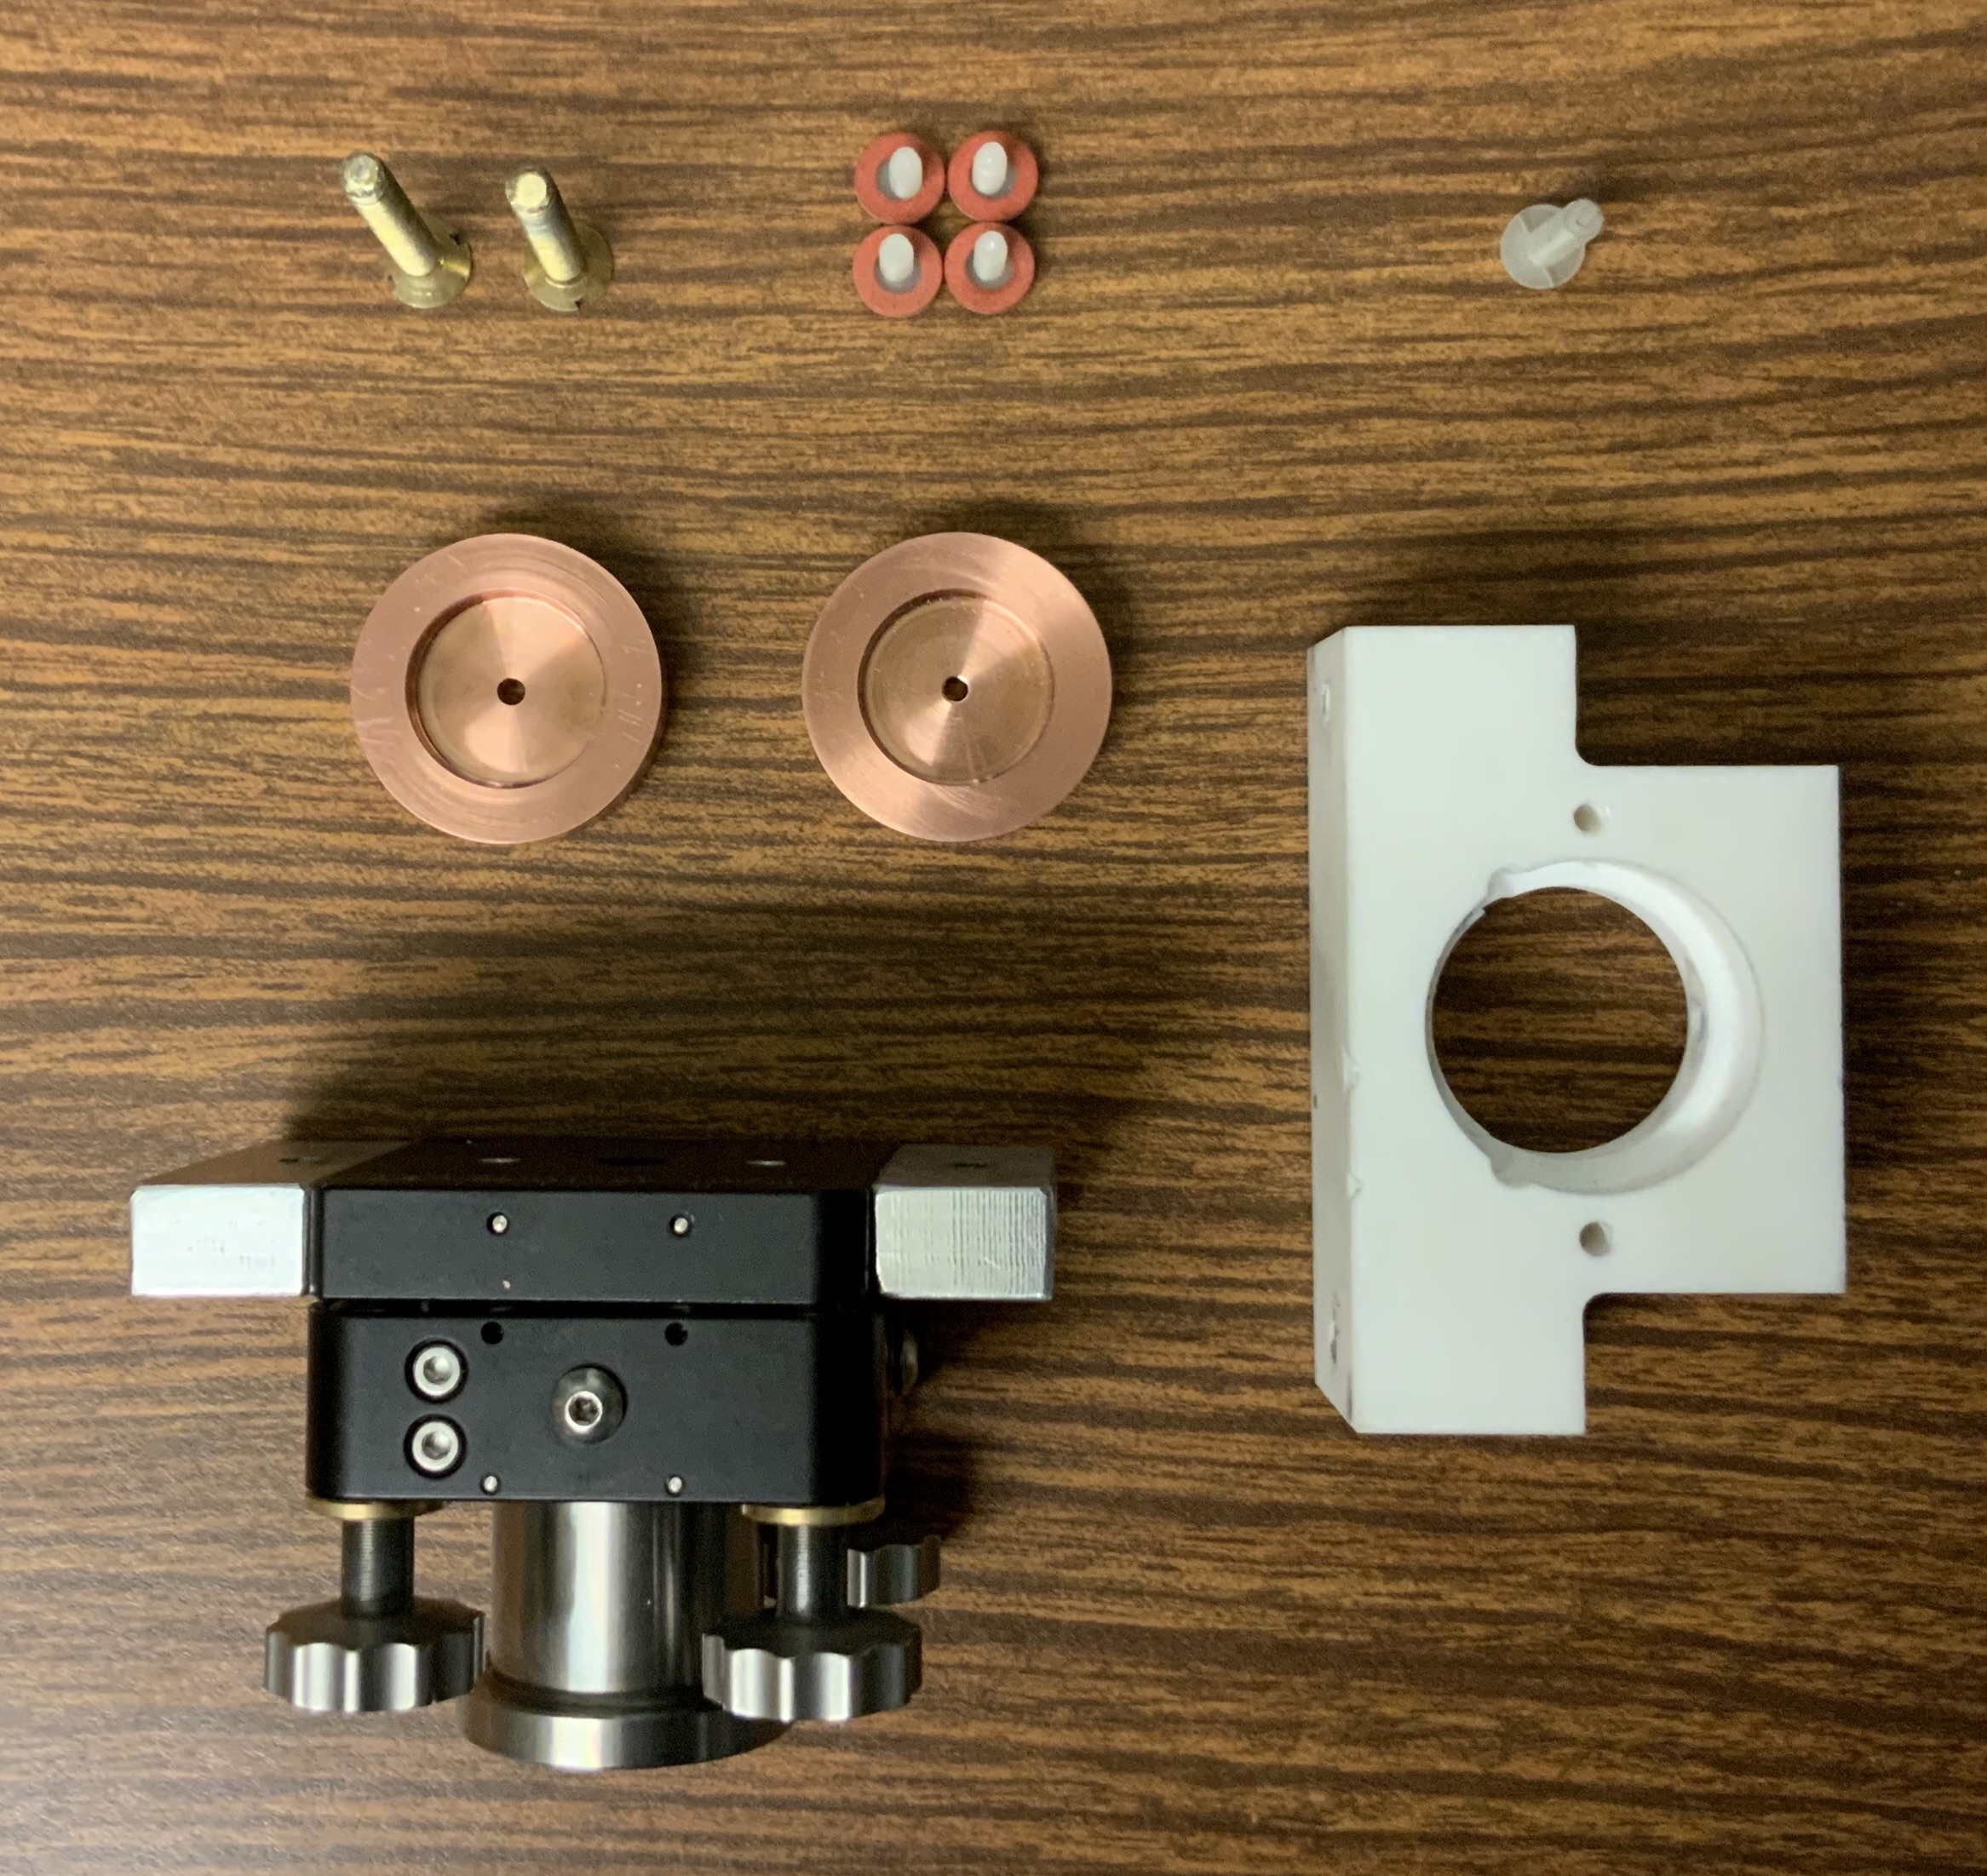
\includegraphics[width=.75\textwidth]{figs/ALGAAS/macor_assembly.jpeg}
\caption{Placeholder for more updated MACOR assembly}
\label{fig:Ez}
\end{figure}
There are two relevant configurations of this experiment: 1) an all-in-one MACOR assembly where the electrodes are mechanically coupled to the optical mount, and 2) larger mechanically decoupled electrode plates.
\\
\textcolor{red}{A lot of time was dedicated towards preliminary mounts made of PLA and PETG. Do I want to do updated measurements and make statements about noise produced from these mounts?}
\\
\subsection{$|E_z|$ strength estimate}
To convey the problem at hand, it is useful to review the illustration seen \textcolor{red}{here (figure showing the the electrode plates, and sample with AlGaAs coating}
\subsubsection{Math}
To find the Electric field screened by the coating we begin with Gauss' Law:

\begin{equation}
\nabla \cdot D = \rho_\mathrm{free}
\end{equation}

For our problem we assume no free charge, but the fused silica substrate with the AlGaAs coating presents dielectric material between the plates. Our initial boundary conditions are also expressed in terms of plate potentials so it is natural to first solve for the potential ($V$) for every point within our system. We can exploit the cylindrical symmetry with the optic and plate geometry in the $r$ coordinate so we shall express the Laplacian accordingly:
\begin{equation}
(1-\chi)\bigg[\frac{1}{r}\frac{\partial}{\partial r} \bigg( r \frac{\partial}{\partial r}\bigg) + \frac{\partial^2}{\partial z^2}\bigg]V = 0
\end{equation}
Where $\chi$ is a spatially dependent electric susceptibility. (\textcolor{red}{Establish coordinates for $\gaas$/$\algaas$, as well as the fused silica substrate so the computation is transparent})
\\
\satoshi{Definition of $\rho$ must be explained. $\rho$ and $\rho_{\mathrm{free}}$ are confusing.
Define $\chi$ and $V$.}
\noindent\textcolor{red}{I will change $\rho$ to $r$ am going to modify figure text so it matches soon.}

Utilizing this, we can proceed to a construction of a numerical Laplacian.

\subsubsection{Numerical approximation}


\begin{itemize}
\item Potential map computation in cylindrical
\item Computing $E_z$ from potential map
\begin{itemize}
\item inside coating
\item outside coating
\end{itemize}
\end{itemize}


\begin{figure}[H]
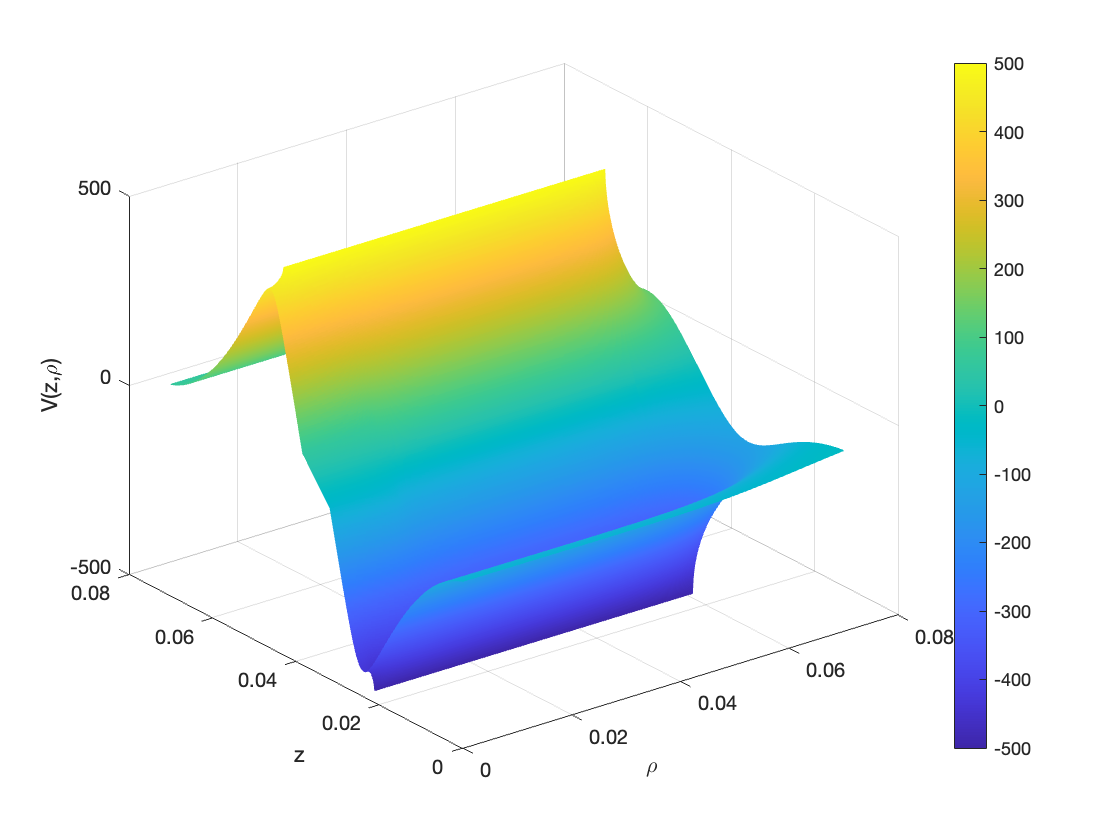
\includegraphics[width=\textwidth]{ALGAAS/13-Sep-2021_potential_map}
\caption{Poisson calculator output potential map ($V(z,r)$ in cylindrical coordinates)}
\label{fig:poisson_calc_output}
\end{figure}

\begin{figure}[H]
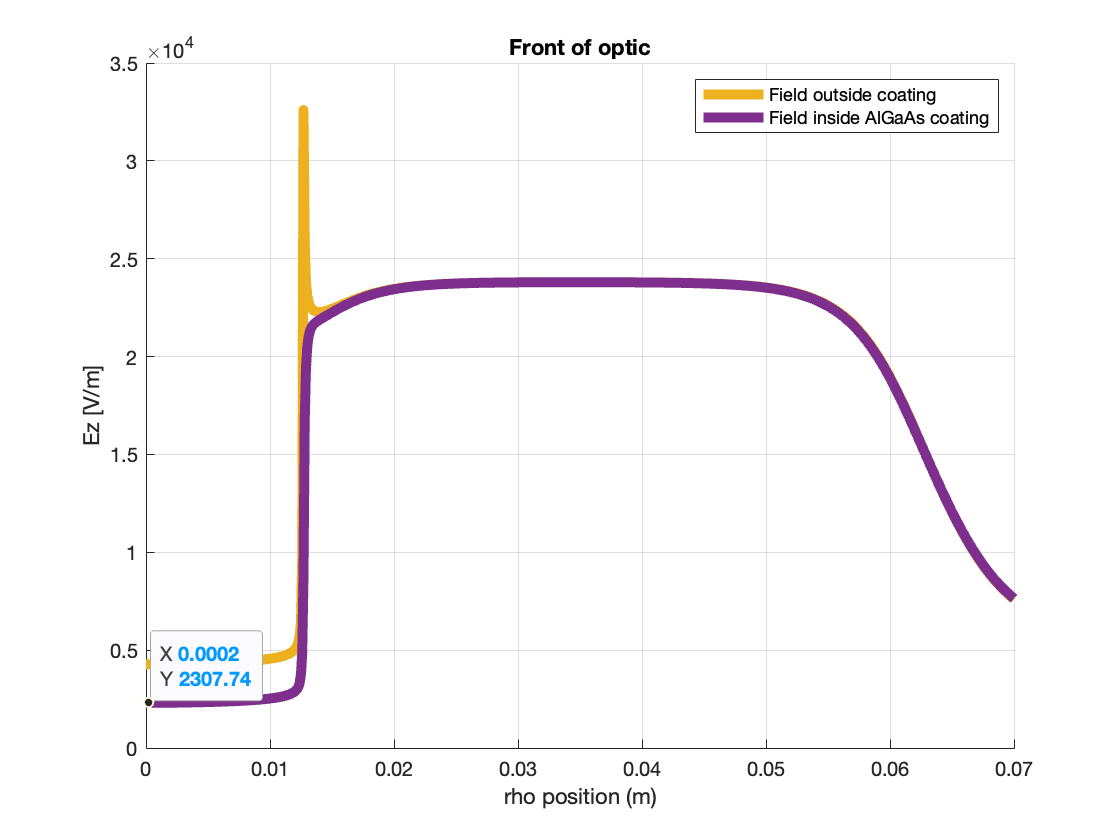
\includegraphics[width=\textwidth]{ALGAAS/13-Sep-2021_e_field_inside_outside_normal}
\caption{$|E_z|$ screened by the scoating and immediately outside AlGaAs coating. \textcolor{red}{Needs to be updated with more current settings}}

\satoshi{How large applied voltage is assumed?}

\label{fig:Ez}
\end{figure}

\begin{figure}[H]
\centering
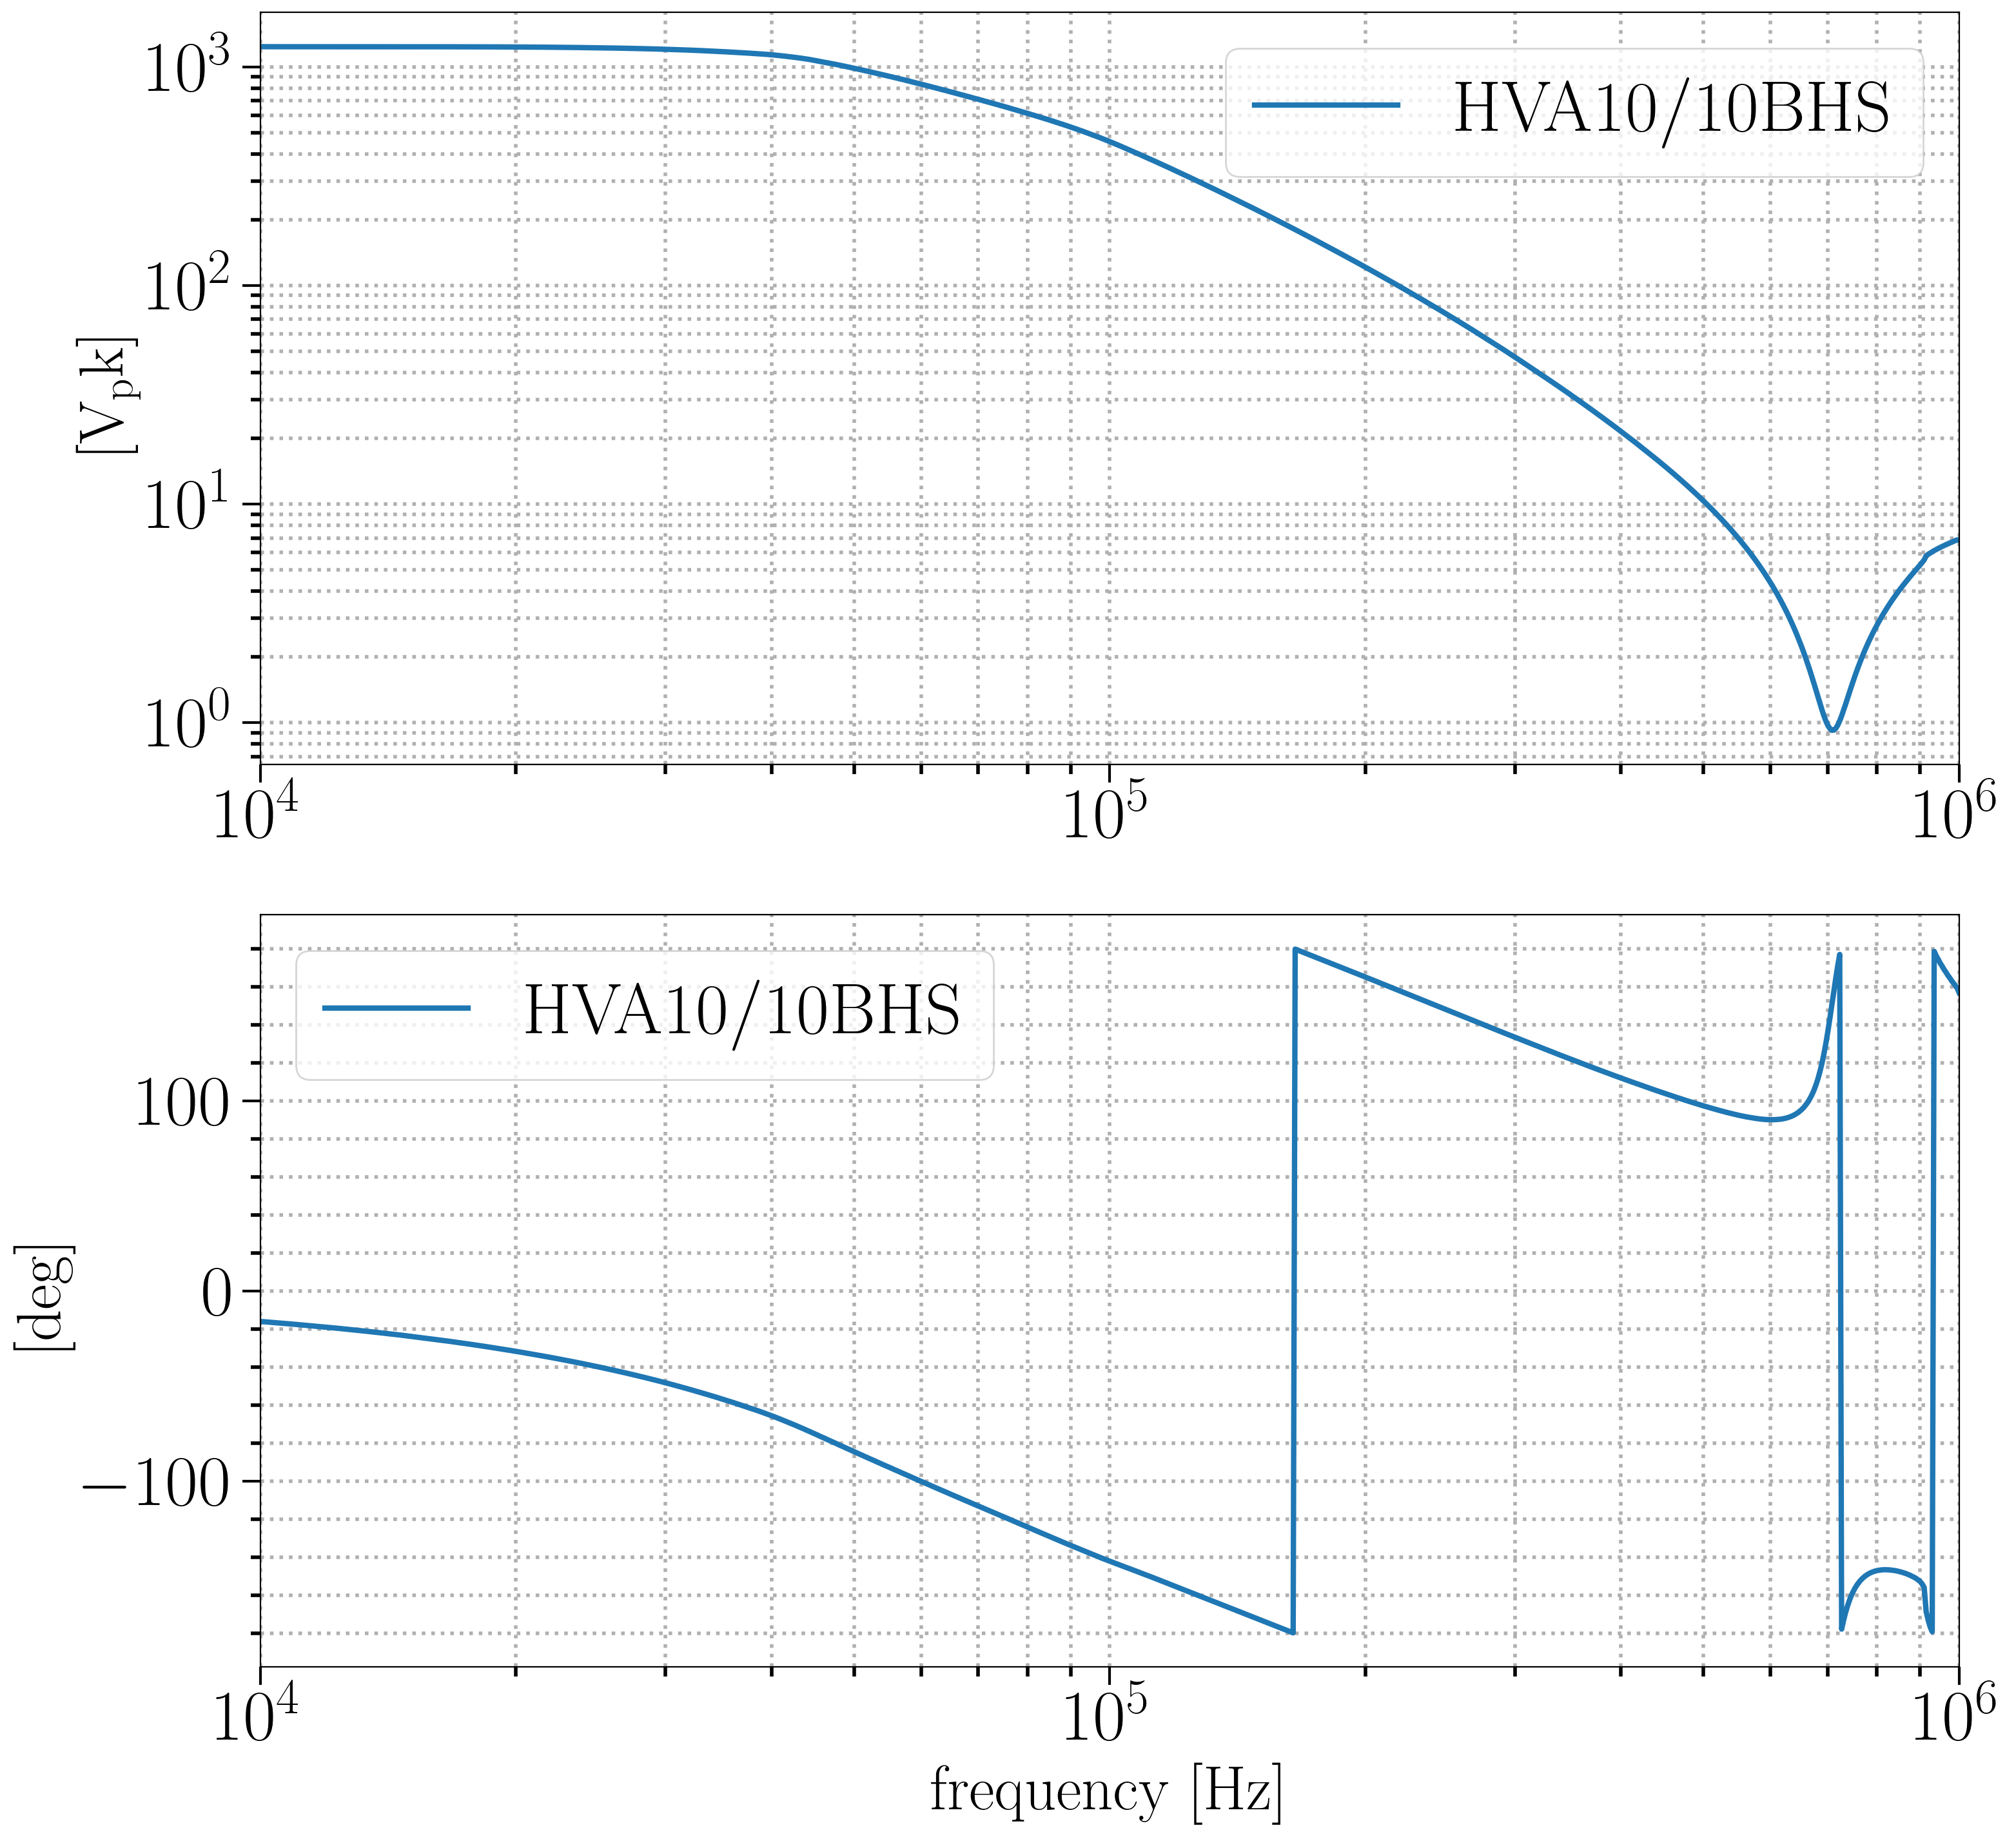
\includegraphics[width=.75\textwidth]{figs/ALGAAS/HVA_TREK1010BHS_1260V_out.png}
\caption{TREK 10/10B-HS HVA frequency dependent measurement. Using Poisson calculator to estimate field strength within coating. (\textcolor{red}{Just HVA for now but will update.} \textcolor{red}{Also, assumes a flat response from coating within this studied region (is this a good assumption or could I do better? (dielectric frequency dependence))}}
\label{fig:Ez}
\end{figure}

\subsection{Calibration}
As discussed, we know that the error signal spectra provides us a voltage spectra that with the above information about the Plant/servo electronics, allows us to
$\mathrm{VFSSOUT}_\mathrm{rms}/\sqrt{Hz} \rightarrow m_\mathrm{rms}/\sqrt{\mathrm{Hz}}$

$$\Delta \mathrm{L} = \mathrm{source}*\alpha(f) \mathrm{A}(f)*\frac{1+\mathrm{OLG}(f)}{\mathrm{OLG}(f)}*\frac{\mathrm{L_{cav}}}{f_\mathrm{laser}}$$

\subsection{Noise Floor}
\subsubsection{Various noise contributions that add up to measured noise floor}
\subsubsection{Shot noise}
Look at the derived shot noise estimate in the appendix V in the Black paper \cite{black_pdh}

\subsubsection{Laser frequency noise}

\begin{itemize}
\item Measure with initial LIGO PMC?
\item There is also a spectra in the Mephisto laser spec sheets
\end{itemize}

\subsubsection{Residual gas noise}

\subsection{Results}

\subsubsection{Mount noise (3D printed mount mechanical noise)}
\subsection{Drive coupling}

\begin{figure}[H]
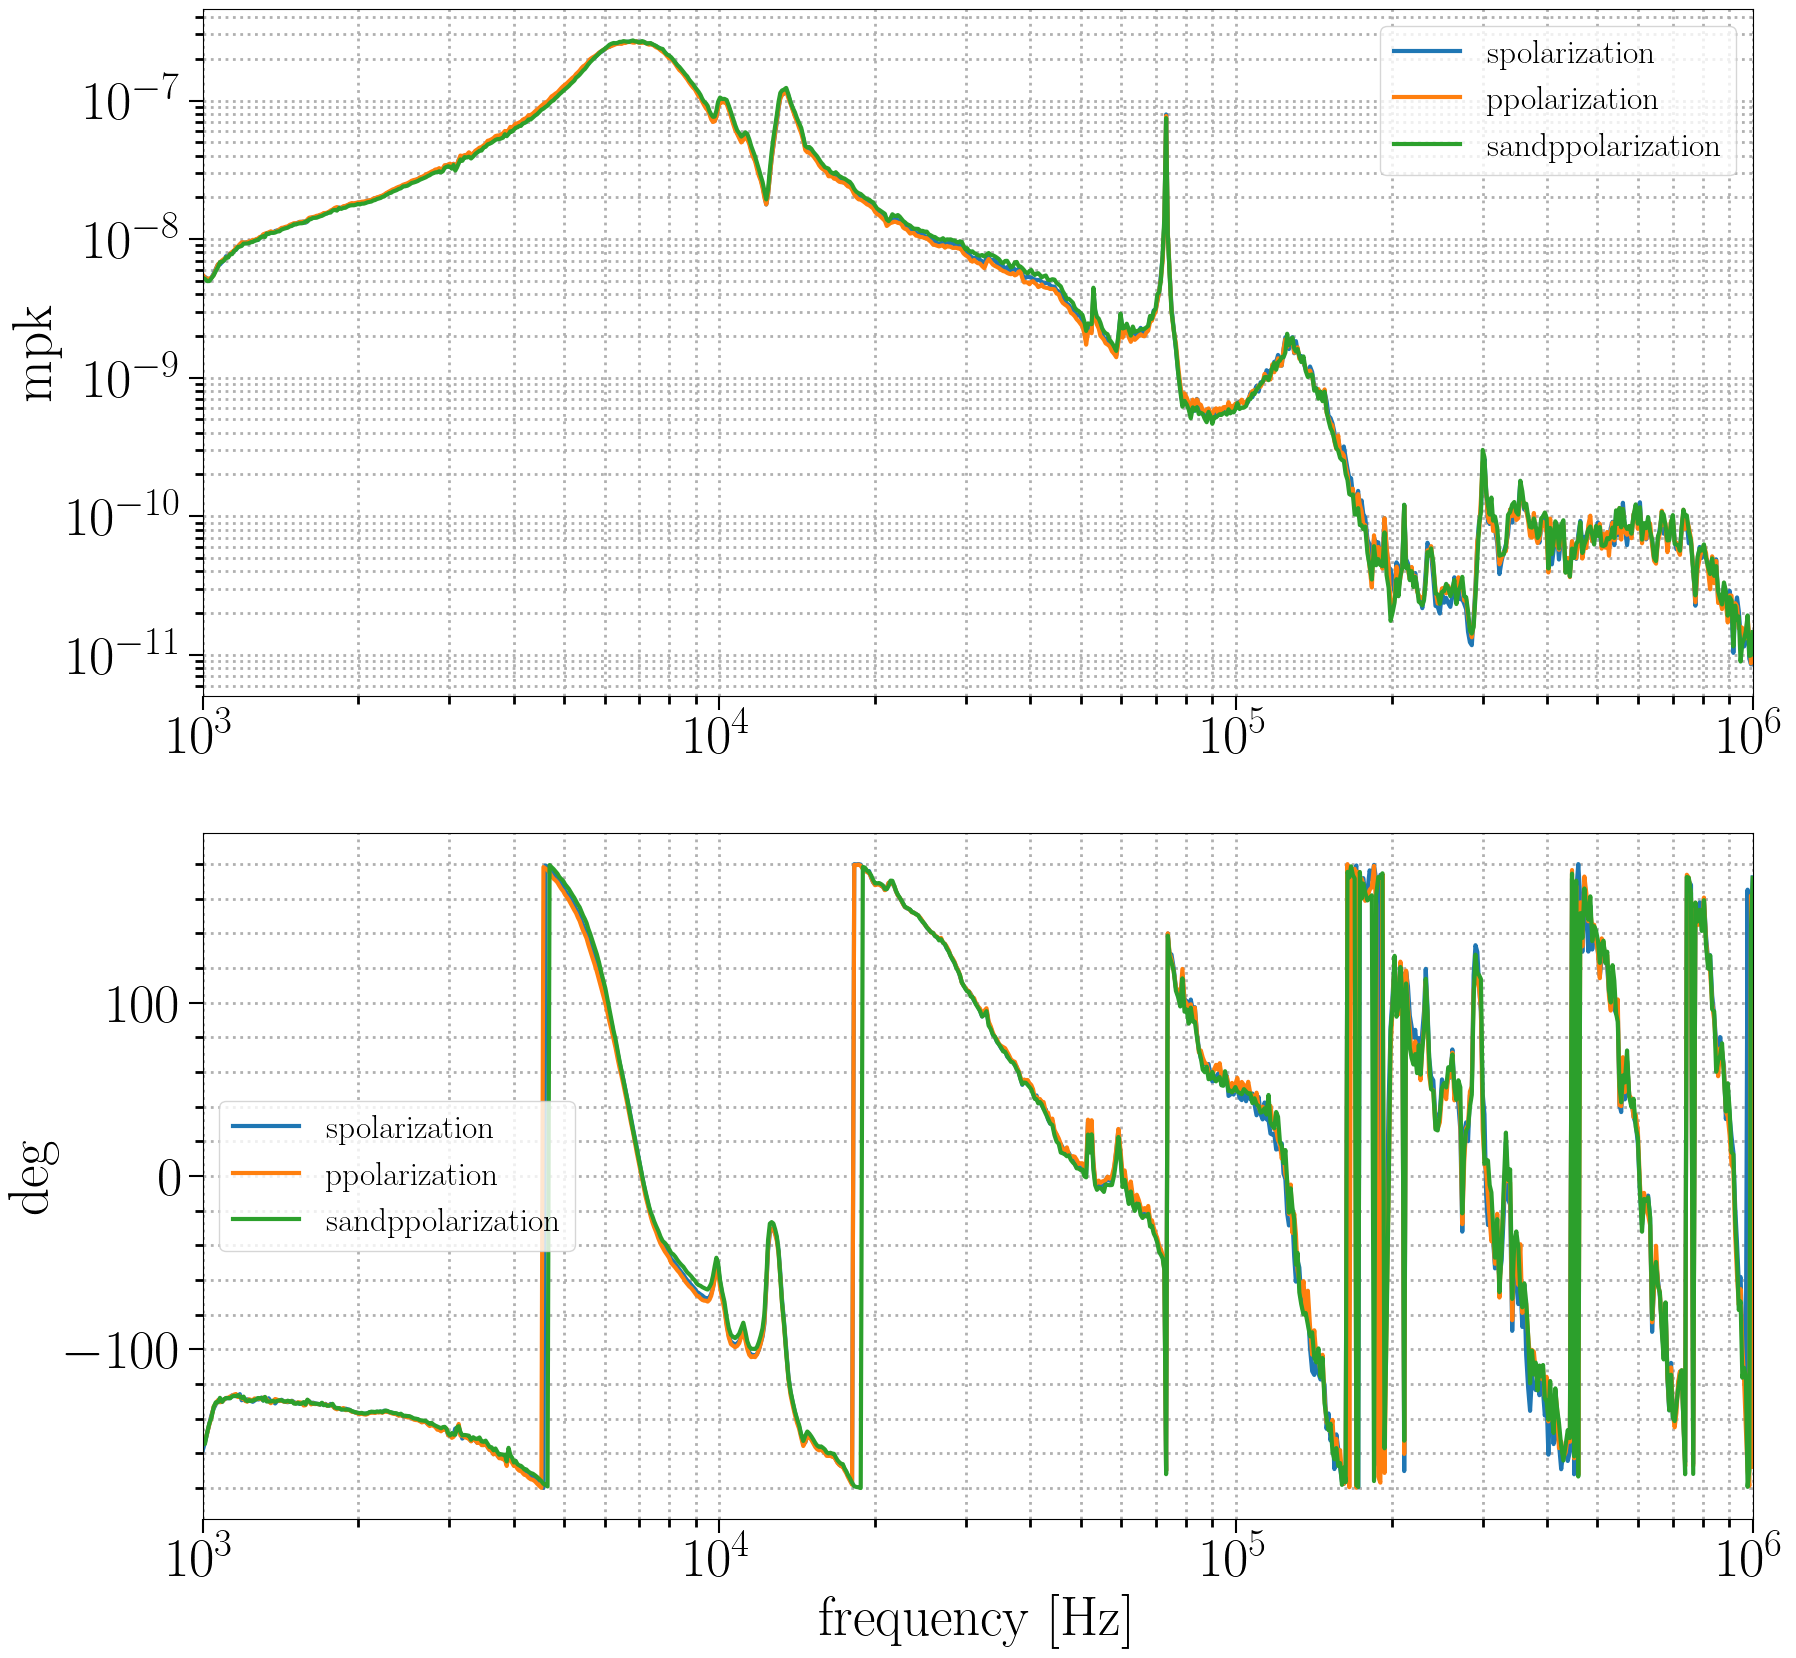
\includegraphics[width=\textwidth]{figs/ALGAAS/cav_polarization_test.png}
\caption{Figure that will include the displacement noise floor, (pockels estimate)*(poisson calculator estimate)*(HVA drive frequency dependence), and the drive coupled measurement \textcolor{red}{figure size needs to be increased}}
\label{fig:measurement_sum}
\end{figure}

\subsubsection{Opto-mechanical coupling}
Sample and mount mechanical mode excitations. Seen with both AlGaAs and a HR coating from an AtFilm (IBS coating)
\begin{itemize}
\item \textbf{Vibration of plates (Leissa)} \cite{leissa} Computing frequencies and order of magnitude
\item \textbf{Steve's COMSOL model results}
\end{itemize}

\subsubsection{Proposed alternative measurement schema}
